\chapter[Mitigating Obfuscation Attacks]{Mitigating Automated Obfuscation Attacks}\label{cha:defense}

As automated obfuscation attacks become increasingly sophisticated, robust defense mechanisms in software plagiarism detection systems are more vital than ever. In this chapter, we address this critical challenge by presenting defense mechanisms to enhance the resilience of these systems against various obfuscation strategies (\contribution{3}). All defense mechanisms discussed in the following apply to any token-based plagiarism detection system. As previously mentioned in \autoref{sec:SPD}, all state-of-the-art approaches used in practice fall into this category. Furthermore, the defense mechanism can also be applied to other structure-based detection approaches with little adaption needed.


The remainder of the chapter is structured as follows.
To effectively mitigate the risks posed by automated obfuscation, we first outline the specific requirements that defense mechanisms must meet.
%
The core of this chapter is dedicated to three novel defense mechanisms, each tailored to counter distinct types of obfuscation attacks:

\begin{description}
    \item[{Token Sequence Normalization}~\cite{Saglam2024b}] (see \autoref{sec:tsn}) utilizes specialized graphs to generate a normalized token sequence that is invariant to insertion- and reordering-based attacks. It combines the benefits of graph-based and token-based approaches by leveraging graph-based techniques to normalize the linear token sequence.

    \item[{Subsequence Merging}~\cite{Saglam2024c}] (see \autoref{sec:smm}) reverses obfuscation attacks by heuristically combining neighboring subsequences matches. Its attack-independent nature allows it to reverse the effects of a broad spectrum of obfuscation attacks, making it applicable to both programming and modeling assignments.

    \item[{Model Subtree Reordering}~\cite{Saglam2024a}] (see \autoref{sec:msr}) is specifically designed for modeling artifacts, such as \ac{EMF} metamodels or \ac{UML} models. The mechanism employs a multi-step algorithm that normalizes the order of nodes in the model tree, effectively countering reordering attacks.
\end{description}

In addition to these primary mechanisms, the chapter also explores other, less effective defense strategies. While these alternative approaches offer some protection, they have notable downsides or are less effective than our primary defense mechanisms.


\ownpublications{
\fancycite{Saglam2024b},
\fancycite{Saglam2024a},\\
\fancycite{Saglam2024d}, and
\fancycite{Saglam2024c}.
}

\section{Requirements}\label{sec:tsn-requirements}
Before we discuss our different defense mechanisms against obfuscation attacks, we want to highlight the key requirements for such mechanisms.
These requirements are directly derived from the obfuscation attack threat model introduced in \autoref{cha:threatmodel}.
%
In addition to these imperative requirements, language dependence is an important factor to discuss, as it greatly affects the applicability of any given defense mechanism.

For any normalization approach to be applicable in real-world scenarios, it must meet the following requirements.
Firstly, it must operate at an {abstract level}, focusing on tokens rather than code.
Furthermore, it must support {explainability}~\cite{Karnalim2021} via traceability between input programs and the computed matches and similarity scores, allowing for the visualization of potential plagiarism with the original, {unaltered program}.
The fact that it is unaltered is essential from both ethical and administrative perspectives~\cite{Simon2016}, as it ensures that the original code remains the basis for human decision-making in plagiarism detection~\cite{Le2013}.
Furthermore, the altered code may no longer contain \textit{idiosyncrasies} (e.g., obvious obfuscation attempts) that assist the decision-making~\cite{Novak2019}.
Consequently, normalization approaches that modify the input programs as pre-processing steps are not applicable.
Existing code normalization approaches, such as dead code elimination with program dependence graphs, do not meet these requirements.

\begin{description}
    \item[Language-Dependence] Implementing a defense mechanism as a pre-processing step for the input programs is language-specific, necessitating a newly designed mechanism for each supported language. This is tedious and costly, and thus, a defense mechanism should be \textit{language-independent}, ensuring versatility across programming languages. However, the more language-independent an approach is, the more abstract the information on which it operates. This abstraction provides a challenge that needs to be addressed to avoid affecting the effectiveness of the defense mechanism. At a minimum, the approaches should be \textit{language-agnostic}, meaning they require some adaption for each language but do not require a complete redesign.
    %Our approach is language-independent, ensuring versatility across languages.
    
    \item[Abstraction Level] For seamless integration into token-based approaches, any defense mechanism must operate at an abstract level, focusing on tokens rather than code, enabling the capture of structural similarities while minimizing the influence of language-specific syntax~\cite{prechelt2002, liu2006, Nichols2019}. 
    %
    This abstraction allows the defense mechanism to generalize across different programming languages, making it versatile and broadly applicable. By focusing on the structural patterns of the code rather than its specific syntax, the mechanism operates on the same level as the detector. This avoids depending on vulnerable information, e.g., variable names or types, that can be used as an additional attack vector.

    \item[Explainability] Any defense mechanism must preserve explainability~\cite{Karnalim2021}, meaning there should always be the ability to understand the similarity score, how it was computed, and which parts of the input programs are similar or dissimilar. This requirement is crucial for maintaining transparency and ensuring educators and other stakeholders trust the detection process. This includes providing clear insights into the matching process and highlighting the code fragments contributing to the final similarity score. In many countries, academic misconduct investigations are led by administrative staff~\cite{Simon2016}. In these cases, explainability is especially critical.

    \item[Preserving Originality] In plagiarism detection, plagiarism detectors must deliver evidence based on the input programs. 
    It becomes difficult to convince non-expert staff when using altered programs as the basis of an argument~\cite{Le2013}. Accused individuals may rightfully assert that the altered programs are not what they originally submitted, thus hindering explainability.
    Moreover, when using pre-processed or altered programs for result visualization, the programs might seem more similar to the human observer than they were initially.
    Thus, the original, unaltered code must be used for human decision-making~\cite{Le2013}.
    Ideally, the subsequence matching and similarity calculation is resilient to obfuscation attacks, but the original, unaltered code is used to visualize these results.
    
    \item[Preserving Idiosyncrasies] Similarly, when the altered code is used for the visualization, some idiosyncrasies of the original programs (e.g., obvious obfuscation attempts) are no longer present. However, these idiosyncrasies are often used as evidence for both initial decision-making and presentation of evidence in misconduct investigations and the related hearing with the students~\cite{Novak2019, Denzler2024}. Hence, relying on altered code renders presenting a compelling argument in a plagiarism case considerably more challenging. It thus negatively affects human decision-making.
    
    \item[Automation] In software plagiarism detection, the similarity calculation must be fully automated to effectively tackle the problem at scale. A defense mechanism that breaks this property and requires human intervention during the pairwise comparison becomes inapplicable at scale. Automation ensures that the defense mechanism can handle the data of large courses efficiently. Human decision-making should only begin once the results are presented, allowing for scalable and efficient plagiarism detection.
     
\end{description}


\section{Token Sequence Normalization}\label{sec:tsn}

In this section, we introduce our first defense mechanism (\contribution{3.1}) called \textit{token sequence normalization}~\cite{Saglam2024b}.
A few years ago, \citet{DevoreMcDonald2020} introduced \textit{\mossad}, a plagiarism generator inspired by genetic programming that allows generating multiple obfuscated versions of a single program.
While most software plagiarism detectors exhibit resilience against some \textit{obfuscation attacks}~\cite{Joy1999,prechelt2000}, \mossad exploits a vulnerability that is inherent in the most widely used approaches.
Although there are graph-based approaches that are potentially less vulnerable to such attacks, they are not feasible in practice~\cite{liu2006} since the subgraph isomorphism problem is NP-complete~\cite{Shang2008, McCreesh2020, Lubiw1981}.

As discussed, \mossad repeatedly inserts statements into the plagiarized program to interfere with the subsequence matching of a potential detector.
To that end, sets of pre-defined statements called \textit{entropy} and existing statements from the original program are used.
The insertion is stopped when the plagiarized instance falls below a certain similarity threshold compared to the original.
%
While \mossad is only one example of an automated obfuscation attack, it is highly effective as similar attacks based on statement insertion are not hard to implement. Thus, it is especially important to provide strong resilience to insertion-based obfuscation.

Token sequence normalization successfully provides resilience against such automatic obfuscation attacks.
It combines the effectiveness of graph-based approaches with the scalability of token-based approaches in a best-of-both-worlds approach\footnote{Subgraph isomorphism for two graphs with $n$ vertices has a runtime complexity of $O(n^n)$. Moreover, the advantage of token sequence normalization is that it has to be performed once per program, not per comparison.}.
We leverage program dependence graphs (PDG)~\cite{ferrante1987} to normalize programs.
However, for real-world applicability, any approach should not be language dependent and operate at an abstract level~\cite{prechelt2002, liu2006, Nichols2019}. Furthermore, it must support explainability via traceability, enabling visualization based on the original, unaltered code.
From both ethical and administrative standpoints~\cite{Simon2016, Le2013}, only the original, unaltered code should inform human decision-making in academic misconduct investigations.
Moreover, the unaltered code often contains idiosyncrasies~\cite{Novak2019} due to obfuscation. They are used for both initial decision-making and misconduct investigations.
Hence, it is not sufficient to eliminate dead code in the input programs.
Existing dead code elimination methods do not fulfill these requirements, as they are fully language-dependent, modify the programs, and are incompatible with ethical and administrative concerns.

In contrast to dead code elimination, our defense mechanism is specifically designed to meet these requirements.
It expands upon the inherent resilience of token-based approaches by making the token sequence virtually invariant against insertion- and reordering-based attacks.
As part of that, we introduce the concept of a \textit{token normalization graph} (TNG), which operates on the token sequence and is thus language-independent.
With that token normalization graph, we normalize the token sequence by removing dead statements and putting subsequent independent statements in a fixed order.
Thus, we effectively reverse the insertion and reordering of statements and de-obfuscate plagiarism instances, thereby achieving high resilience to automatic plagiarism based on these attacks.

\begin{factsheet}{Overview: Token Sequence Normalization} 
    \begin{description}[style=multiline,leftmargin=5.5cm]
        \item[Core Principle] Normalize Token Sequence \\via Graph-Based Representation
        \item[Targeted Obfuscation Attack] Statement Insertion, Statement Reordering
        \item[Language Family] Programming Languages
        \item[Language Dependence] Language-Agnostic
        \item[Performance Impact] Low
        \item[Main Scalability Determinant] Size of Input Programs 
        \item[Integration Complexity] Moderate
    \end{description}
\end{factsheet}

\subsection{Targeted Obfuscation Attacks} \label{sec:icseb:RunningExample}

Token sequence normalization is designed to defend against two particular obfuscation attack types: Semantic-preserving statement insertion and statement reordering. These attacks aim to affect the token sequence derived from a program by modifying the program without changing its underlying behavior, thereby misleading plagiarism detection tools. %Two primary forms of targeted obfuscation attacks are considered: reordering of independent statements and insertion of (dead) statements.

%\subsubsection{Insertion of (Dead) Statements}
A simple yet effective obfuscation attack is the insertion of dead statements. Dead statements are lines of code that do not affect the program's output or behavior. These can include redundant assignments, unused variables, or code blocks that are never executed (e.g., due to always-false conditions). An attacker can significantly alter the token sequence without changing the program's functionality by inserting such statements at various points in the code. Furthermore, dead statements can be obfuscated themselves by inserting further statements that depend on them.

\begin{samepage}
\begin{lstlisting}[caption={Example for Obfuscated Dead Statements},label=lst:complexinsertion]
int x = 10;
boolean checked = false; // Dead statement
int y = 5;
if (checked) { // Dead block, only depends on the dead statement
    y = 20;
}
println(x + y);
\end{lstlisting}
\end{samepage}

\autoref{lst:complexinsertion} illustrates such a dependence between inserted statements. Both the variable \texttt{checked} and the control structure are dead code. However, the variable is referenced as a condition of the control structure.
However, as these statements do not alter the behavior of the program, they are still dead code. However, it is harder to detect them, as statement interdependence has to be fully resolved.

%\subsubsection{Reordering of Independent Statements}
Reordering independent statements involves changing the order of code statements that do not depend on each other, meaning the order of the statements does not affect the behavior of the program. This type of obfuscation leverages the fact that most programming languages allow statements that do not affect each other's execution order to be rearranged. For example, swapping the order of two variable assignments that do not depend on each other's values is possible. This attack is considered a weak form of obfuscation, as the degree of freedom to reorder statements in most programs is limited. Only some statements can be reordered, thus making it challenging to apply this obfuscation broadly.

Both statement insertion and reordering can be automated in different ways. Our defense mechanism is designed to counter these attacks independent of their automation, be it \mossad-style random obfuscation until a certain threshold is reached or exhaustive obfuscation where the obfuscation is applied to all possible code positions.

\noindent
As a combined running example for both insertion and reordering, we introduce the programs shown in \autoref{tab:codesnippet}. 
Both programs print the squared values of the numbers from 1 to 10.
The right program is a modified variant based on two changes that alter its structure.
Thus, the program still behaves the same upon execution.
In detail, line 3 was inserted in the modified variant, and lines 6 and 7 were swapped.
%Minimal example, no focus on renaming as popular code plagiarism detectors are resilient by using abstraction \cite{} 
%Also, there is no focus on deletion, as it is not practical if functionality should not be reduced
While the relationship between the programs is evident in this simple example, this is not true for larger programs that undergo extensive modifications to obfuscate the relation between the variant and the original. Thus, these modifications can be used to conceal plagiarism. 
Additionally, manual comparison becomes infeasible when dealing with numerous student submissions, even for smaller programs.
However, for plagiarism detectors, structural obfuscation attacks like these diminish the detection quality~\cite{DevoreMcDonald2020}. 
%Easy to detect, but only minimal example. Large-scale obfuscation in thousands of lines with hundreds of submissions, easy to be overlooked

To illustrate this, \autoref{tab:tokens} shows the token sequences of the two programs in \autoref{tab:codesnippet}.
While the structural information concerning method context, loop context, declarations, and assignments remains intact, specific details such as names, types, or comments are excluded.
Note that the changes lead to two sequences that are different enough to affect the detection quality, as only shorter subsequences can be matched between them. In detail, we can find three matching subsequences of length two: The first two lines, the last two lines, and finally, lines four and five. As discussed, these subsequences are short enough to fall below the plagiarism detector's threshold.

\begin{samepage}
\begin{table}
	\centering
	\begin{tabular}{rlcl}
		\toprule
		\textbf{\#} & \textbf{Original}                              &                  & \textbf{Variant}                                   \\
		\midrule
		1           & \texttt{~~void printSquares() \{}              &                                    & \texttt{~~void printSquares() \{}                  \\
		2           & \texttt{~~~~int i = 1;}                        &                                    & \texttt{~~~~int i = 1;}                            \\
				
		3           &                                                & \small\textbf{\phantom{$\to$}  insert $\to$} & \cellcolor{add}\texttt{~~~~boolean debug = false;} \\
				
		4           & \texttt{~~~~while (i <= 10) \{}                &                                    & \texttt{~~~~while (i <= 10) \{}                    \\
		5           & \texttt{~~~~~~int square = i * i;}             &                                    & \texttt{~~~~~~int square = i * i;}                 \\
		6           & \cellcolor{del}\texttt{~~~~~~println(square);} & \small\textbf{$\to$ reorder $\to$} & \cellcolor{add} \texttt{~~~~~~i++;}                \\
		7           & \cellcolor{del}\texttt{~~~~~~i++;}             & \small\textbf{$\to$ reorder $\to$} & \cellcolor{add} \texttt{~~~~~~println(square);}    \\
		8           & \texttt{~~~~\}}                                &                                    & \texttt{~~~~\}}                                    \\
		9           & \texttt{~~\}}                                  &                                    & \texttt{~~\}}                                      \\
		\bottomrule
	\end{tabular}
    \caption[Example Obfuscation: Insertion and Reordering]{Original code (left) and modified variant (right) after inserting one statement and reordering two. Removed lines are highlighted in red, and added lines are highlighted in green.}
	\label{tab:codesnippet}
\end{table}


\begin{table}
    \centering
    %\small
    \begin{tabular}{c@{\hskip 15pt}l@{\hskip 30pt}c@{\hskip 30pt} r}
        \toprule
        \# & \textbf{Original Tokens}     &                     & \textbf{Variant Tokens}      \\
        \midrule
        1  & \texttt{method start} &                 & \texttt{method start} \\
        2  & \texttt{variable}     &                 & \texttt{variable}     \\
        3  &                       & \textbf{\phantom{$\to$}  insert $\to$}    & \cellcolor{add}\texttt{variable}     \\
        4  & \texttt{loop start}   &                 & \texttt{loop start}   \\
        5  & \texttt{variable}     &                 & \texttt{variable}     \\
        6  & \cellcolor{del}\texttt{apply}        & \textbf{$\to$  swap $\to$} & \cellcolor{add}\texttt{assignment}   \\
        7  & \cellcolor{del}\texttt{assignment}   & \textbf{$\to$  swap $\to$} & \cellcolor{add}\texttt{apply}        \\
        8  & \texttt{loop end}     &                 & \texttt{loop end}     \\
        9  & \texttt{method end}   &                 & \texttt{method end}   \\
        \bottomrule
    \end{tabular}
    \caption[Example Obfuscation Tokens: Insertion and Reordering]{Comparison of the original and obfuscated token sequences corresponding to the program statements in \autoref{tab:codesnippet}. One token is inserted at index 3, while two tokens at indices 6 and 7 are swapped.}
    \label{tab:tokens}
\end{table}
\end{samepage}

\subsection{Concept}

The defense mechanism is an additional step in the pipeline of a plagiarism detector before the pairwise comparison, which effectively de-obfuscates plagiarism for the remaining steps in the pipeline.
At a high level, our mechanism operates as follows for each input program:

\begin{enumerate}
    \item We enrich the token sequence with additional language-agnostic semantic information about the interdependence of the tokens.
    \item We construct a language-independent graph-based representation of the tokenized program from the enriched token sequence, which abstracts from the original code. This graph represents a partial order of the tokens.
    \item We then use this graph to generate a normalized token sequence, thus effectively reverting insertions and reordering operations.
    \begin{enumerate}
        \item Insertions are countered via subsequence removal.
        \item Reordering is negated by topological sorting~\cite{kahn1962}.
    \end{enumerate}
    \item The comparison is still conducted exclusively on the token sequence, circumventing the computational complexity of graph-based approaches.
\end{enumerate}

\noindent
We call the representation of the tokenized program a \textit{token normalization graph} (TNG).
Each node in this graph represents the tokens of a program statement.
As it is based on the token sequence, it is language-independent, which enables our defense mechanism to be applicable to any programming language.
Thus, the format of the semantic information utilized to enrich the token sequence must also be language-independent.
%
We specify a generic format for the semantic information based on the interdependence between tokens that abstracts from the detail of the underlying programming language.
The semantic information must be extracted from the input programs alongside the tokens.
Therefore, the extraction needs to be implemented separately for each language the detector supports.
It is the sole language-dependent step that our defense mechanism adds.
While the format of the semantic information and the TNG is language-independent, the need to provide this information makes the defense mechanism language-agnostic.
However, extracting semantic information does not impose additional constraints on the detector since tokenization is inherently language-dependent.


\subsection{Semantic Information}

\label{subsec:semantic}
In order to construct a TNG, we need information about the interdependencies between the tokens.
This information is not present in the token sequence and thus must be additionally attached to the tokens.
To that end, a language-independent format is required for this semantic information.
Using this format, the tokens can be automatically annotated during their extraction from the parse tree. Different types of statements lead to different types of information.
Thus, this format allows us to map the relations of the statements in the program to the tokens independent of the underlying language of the program.
%
We specify the following format for this semantic information:
%\begin{samepage}
\begin{description}
    \item[Criticality] describes statements that contribute to programs' behavior through means other than variables and thus must not be removed. Therefore, a token can be either critical or not critical.
        \textit{In our example in \autoref{tab:codesnippet}, the critical statements are the \texttt{while} statement and the \texttt{println} statement. Thus, the \texttt{loop start} and \texttt{apply} tokens in \autoref{tab:tokens} are critical.}
    \item[Fixed Order] describes how statements must maintain their relative order to ensure semantic equivalence. Tokens can thus be either fixed in their order or non-fixed. Fixed order tokens act as reordering boundary, as preceding tokens cannot be moved after this boundary and vice versa.
        \textit{In the running example, the \texttt{while} statement dictates that the statements within the loop cannot be moved outside the loop. Thus, the loop tokens of lines 4 and 8 in \autoref{tab:tokens} are fixed order tokens.}
    \item[Variable Access] describes the variable accesses (read or write) for each statement, thus indicating on which other statements they depend.
        Hence, each token has two variable identifier sets: One for read accesses and one for write accesses.
        \textit{In the running example, the \texttt{while} statement depends on the statement the declares the variable \texttt{i}. Therefore, the \texttt{loop start} token contains \texttt{i} in its read access set.}
    \item[Loop] describes statement blocks in which the execution order of the statements can deviate from their declaration order. Therefore, the first and last tokens corresponding to the loop are marked with loop start and loop end flags.
        \textit{In the running example, the statements in the loop body are repeatedly executed. Thus, the incrementation of the variable \texttt{i} may be executed not only after the \texttt{println} statement but also before due to the repeated execution. In the running example, both \texttt{loop start} and \texttt{loop end} are marked with the loop flag.}
\end{description}
%\end{samepage}


\subsection{Token Normalization Graph}

We use the token normalization graph (TNG) as the underlying data structure to generate a normalized token sequence.
A TNG is a specialized version of a program dependence graph (PDG).
It is designed for tokens instead of code and through a higher abstraction level not confined to the programming language's syntax. Thus, a TNG crucially provides language independence. A TNG contains additional edges required for the token sequence normalization.
While a PDG focuses only on statement dependencies in code, the TNG considers both token interdependence and the order of the tokens. Both are required for token-based approaches.

We construct the TNG from the token sequence and the additional semantic information.
A TNG node represents a single statement and contains all tokens generated from that statement.
After the construction of the TNG, we no longer need the original token sequence.
%
More formally, a token normalization graph is a directed graph \( G = (V, E) \) used to represent the tokenized form of a program for the purpose of normalization. Each node \( v \in V \) represents a statement in the program and contains a subsequence of tokens. Let \( (t_i) \) be the sequence of all tokens in the program. Each statement \( S \) corresponds to a subsequence \( (s_j) \sqsubseteq (t_i) \) where \( (s_j) \) is the set of tokens extracted for \( S \). Thus, each node in the TNG is represented by a subsequence of tokens.
%
The TNG has three types of directed edges, each capturing different dependencies between the statements represented by the nodes:
\begin{description}
    \item[Variable Flow Edges] indicate that a statement writes to a variable that another statement reads. They are similar to the data dependencies in the PDG.
    \textit{A directed edge \( (v_i, v_j) \in E \) is a variable flow edge $(v_i, v_j) \in E_{vf}$ if statement \( S_i \) of $v_i$ writes to a variable that statement \( S_j \) of $v_j$  reads. This edge indicates a data dependency where \( v_j \) depends on \( v_i \) for the value of the variable.}
    
    \item[Variable Order Edges] indicate that altering the order of the two statements may alter variable values and, thus, the program's behavior.
    This edge helps maintain the correct execution order of statements.
    Wherever there is a variable flow edge, there is also a variable order edge; however, not necessarily in the same direction.
     \textit{A directed edge \( (v_i, v_j) \in E \) is a variable order edge $(v_i, v_j) \in E_{vo}$ if changing the relative order of statements \( S_i \) and \( S_j \) could alter the program's behavior due to variable dependencies.}
     
    \item[Fixed Order Edges] indicate that altering the order of the two statements may affect the program's behavior for reasons beyond variable value alterations.
    This edge enforces the preservation of the original order of critical statements.
    \textit{A directed edge \( (v_i, v_j) \in E \) is a fixed order edge $(v_i, v_j) \in E_{fo}$ if changing the order of statements \( S_i \) and \( S_j \) could affect the program's behavior for reasons other than variable dependencies.}   
\end{description}

\noindent
The TNG is then constructed as follows:
First, we group all tokens within a statement as nodes. %, and edges are then formed based on the tokens' semantic information.
For each statement \( S \) in the program, create a node \( v_i \) containing the subsequence of tokens \( (s_j) \sqsubseteq (t_i) \).
Next, we label nodes containing at least one critical token as \textit{critical}.
We then use the tokens marked as \textit{fixed order} to create fixed order edges $E_{fo}$.
For each node with fixed order tokens, we create incoming and outgoing edges to and from all preceding and subsequent nodes, as determined by the original order of the tokens.
We employ the variable access sets and loop flags to create variable flow edges $E_{vf}$.
Finally, disregarding loop flags, we determine variable order edges $E_{vo}$ solely by variable access sets.
Once the TNG is complete, it contains all the necessary data for generating a normalized token sequence. Thus, the original token sequences can be safely discarded.
Moreover, as for all token-based approaches, the original programs are no longer required for the similarity calculation.


\begin{figure}
\centering
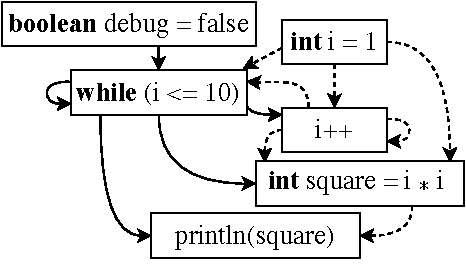
\includegraphics[width=0.5\linewidth]{figures/pdg.pdf}
\caption[Program Dependence Graph]{Program dependence graph of the running example showing control dependencies (solid arrows) and data dependencies (dashed arrows).}
\label{fig:pdg}
\end{figure}


\autoref{fig:pdg} shows a PDG for the plagiarized program in \autoref{tab:codesnippet}. The control and data dependencies between the different code statements are represented via edges.
While the dead statement for the variable called \texttt{debug} can be identified, it cannot be used to generate a normalized token sequence due to the requirements mentioned in \autoref{sec:tsn-requirements}.
\autoref{fig:tng} shows the TNG for the same program. In contrast to the PDG, the nodes represent tokens instead of code. The TNG contains the three types of edges based on the semantic information discussed in \autoref{subsec:semantic}. The two nodes with a gray background are marked as critical. Furthermore, the semantic information of the corresponding tokens is illustrated in the bottom right corner of the node. 
The semantic information is only depicted for the sake of clarity. It is used to construct the TNG but is no longer necessary for the normalization thereafter.

\begin{figure}
\centering
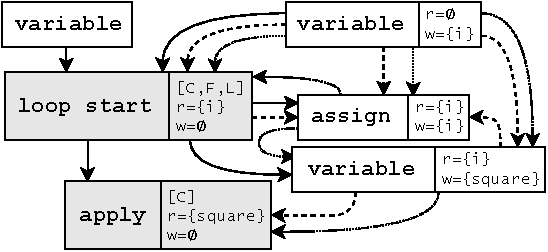
\includegraphics[width=0.6\linewidth]{figures/tng3.pdf}
\caption[Token Normalization Graph]{Token normalization graph for the PDG in \autoref{fig:pdg}, fixed order edges (solid), variable order edges (dashed), and variable flow edges (dotted).
The critical (C), fixed-order (F), and loop (L) flags, with the variable access sets (r for read, w for write), are included for illustrative purposes.}
\label{fig:tng}
\end{figure}


\subsection{Generating the Normalized Token Sequence}

After constructing the TNG, we can leverage it to generate a normalized token sequence in two steps.
%We do so in two steps: One for reverting insertions and one for reverting reordering.
First, we remove all dead nodes. These are all nodes from which no critical node can be reached via variable flow edges $E_{vf}$. This effectively reverts insertions into the token sequence.
Next, we remove all variable flow edges $E_{vf}$ from the TNG, making it acyclical. They have served their purpose for the dead node removal and are no longer required.
In our running example in \autoref{tab:codesnippet}, the statement containing the variable named \texttt{debug} is considered dead code, and so is its corresponding \texttt{variable} node in the TNG in \autoref{fig:tng}.
This node will be removed, as it has no outgoing variable flow edge.
\autoref{tab:tokens-full} illustrates how that affects the normalized token sequence. The code insertion leads to an additional token in the obfuscated token sequence. However, after the dead node removal, this effect is reversed.
\autoref{fig:tng2} illustrates the TNG from \autoref{fig:tng} with the dead node removed and variable flow edges $E_{vf}$ omitted. The previous cycles, such as the one between the \texttt{loop start} and \texttt{assign} nodes, are no longer present.
A partial order becomes apparent when considering the topmost \texttt{variable} node as the root.

\begin{figure}[b]
\centering
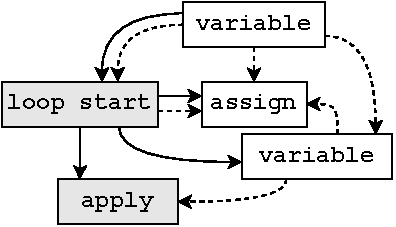
\includegraphics[width=0.45\linewidth]{figures/tng2b.pdf}
\caption[Reduced Token Normalization Graph]{Token normalization graph after the dead nodes and removal of variable flow edges, still present are fixed order edges (solid) and variable order edges (dashed).}
\label{fig:tng2}
\end{figure}

Next, we use topological sorting~\cite{kahn1962} to generate a normalized token sequence. This counters attempts to reorder the token sequence.
Specifically, we order the tokens of the remaining nodes by their node's distance to the aforementioned root.
Nodes with the same distance represent subsequent independent statements. We sort them via the types of tokens in the nodes.
This is a robust criterion, as the extracted tokens are invariant to lexical modifications~\cite{prechelt2002}.
Note that if two nodes with the same root distance are equal according to that criterion, they contain the same tokens, and their order does not affect the normalized token sequence. %; therefore, we can consider them equal in order.

In our running example in \autoref{tab:codesnippet}, statements 6 and 7 were swapped.
\autoref{tab:tokens-full} illustrates how this obfuscation affects the token sequence.
When using the reduced TNG in \autoref{fig:tng2} to generate the normalized token sequence, the sequence after the topological sorting will be identical to the original one (see \autoref{tab:tokens-full}). Thus, the plagiarism detector computes a 100\% match for our running example, despite the obfuscation attempt shown in \autoref{tab:codesnippet}.
Our approach only normalizes the tokens sequence. The original, unaltered code, with all its idiosyncrasies, is used for the visualization. However, as a result of our normalization, the similarity calculation and code matching are not compromised by obfuscation attacks.




\begin{table}
    \centering
    \begin{tabular}{c@{\hskip 12pt}c@{\hskip 4pt}c@{\hskip 4pt}c@{\hskip 4pt}c@{\hskip 4pt}c@{\hskip 4pt}c@{\hskip 4pt}c}
        \toprule
        \# & \textbf{Original} & $\to$ & \textbf{Obfuscated} & $\to$ & \textbf{Nodes Removed} & $\to$ & \textbf{Top. Sorted} \\
        \midrule
        {1}  & \texttt{method start} & & \texttt{method start} & & \texttt{method start} & & \texttt{method start} \\
        {2}  & \texttt{variable}     & & \texttt{variable}     & & \texttt{variable}     & & \texttt{variable}     \\
        {3}  &                                  & \textbf{(+)} & \texttt{\textbf{variable}}     & \textbf{(--)} & & &  \\
        {4}  & \texttt{loop start}   & & \texttt{loop start}   & & \texttt{loop start}   & & \texttt{loop start}   \\
        {5}  & \texttt{variable}     & & \texttt{variable}     & & \texttt{variable}     & & \texttt{variable}     \\
        {6}  & \texttt{apply}        & \textbf{(\textasciitilde)} & \texttt{\textbf{assignment}}   & & \texttt{\textbf{assignment}}   & \textbf{(\textasciitilde)}& \texttt{apply}   \\
        {7}  & \texttt{assignment}   & \textbf{(\textasciitilde)} & \texttt{\textbf{apply}}        & & \texttt{\textbf{apply}}        & \textbf{(\textasciitilde)}& \texttt{assignment}        \\
        {8}  & \texttt{loop end}     & & \texttt{loop end}     & & \texttt{loop end}     & & \texttt{loop end}     \\
        {9}  & \texttt{method end}   & & \texttt{method end}   & & \texttt{method end}   & & \texttt{method end}   \\
        \bottomrule
    \end{tabular}
    \caption[Token Sequence Normalization]{Comparison of the original and obfuscated token sequences with the obfuscated one after the two steps dead node removal and topological sorting \autoref{tab:codesnippet}.}
    \label{tab:tokens-full}
\end{table}


\subsection{Complexity}

The runtime complexity of token sequence normalization depends on extracting the semantic information, creating the token normalization graph, and generating the normalized token sequence.
The semantic information can be extracted during the tokenization step of the plagiarism detector and does not occur at an additional cost.

For the other steps, the runtime complexity depends on the density of the graph and, thus, on its number of nodes, which is limited by the number of tokens $m$ and its number of edges $e$.
As for a PDG, building a TNG can take $O(m^2)$ time in the worst case due to dense dependencies among tokens.
Pruning dead nodes requires a reachability analysis using a graph traversal with a $O(m + e)$ complexity. Topological sorting is performed on the resulting TNG and takes $O(m + e)$ time.

Therefore, the overall runtime complexity is $O(m^2)$ in the worst case (for dense graphs) and $O(m + e)$ in the best case (for sparse graphs).
Note that this has to be done for every input program but not for every comparison, which is a strong advantage compared to graph-based plagiarism detection methods. Thus, doing so for $n$ programs of maximum $m$ tokens has a worst-case complexity of only $O(nm^2)$. Thus, the size of the input programs has a larger impact on the performance of the token sequence normalization than the number of programs.
%
As the worst-case runtime complexity for greedy string tiling for $n$ programs with $m$ tokens, each is \( O(n^2m^3) \) (see \autoref{sec:found-jplag}), token sequence normalization does not increase the runtime complexity of the plagiarism detection process.


\subsection{Observed Impact}
This section presents initial observations on the effectiveness of token sequence normalization based on real-world data. It is important to note that this is not intended as a comprehensive evaluation but instead aims to provide an empirical perspective on how the defense mechanism performs in practical scenarios.

When applying token sequence normalization in practice, we can observe that it effectively renders obfuscation attacks based on insertion and reordering ineffective.
Remarkably, the similarity of unrelated solutions remains virtually unaltered, with an average similarity increase of less than 1\%, effectively avoiding an increase in false positives.
Our defense mechanism comes with a negligible runtime overhead of mere seconds for large real-world datasets, thus showing its practicality.

\autoref{fig:tsn-impact} illustrated the effectiveness of our approach in preventing obfuscation statement insertion.
The solid lines show how the similarity computed by JPlag decreases the more statements proportionally to the input program size are inserted.
Without our defense mechanism, the similarity values drop below 10\%. This renders successful plagiarism detection ineffective, as plagiarized programs can no longer be distinguished from original ones.
To achieve such a low threshold, approximately 50-60\% additional statements need to be inserted.
Note that we employed PlagGen~\cite{Broedel2023} for the obfuscation, which uses an exhaustive strategy. Thus, the input program determines how many statements can be inserted. 

The dashed lines show the same input programs but with token sequence normalization enabled. 
There, the similarity values surge to over 99\%. These results would raise strong suspicions, as for its dataset, the average similarity of unrelated programs is around 10\%. Thus, token sequence normalization renders the obfuscation attack ineffective, making the detector resilient against these attacks.

\begin{figure}[ht]
    \centering
    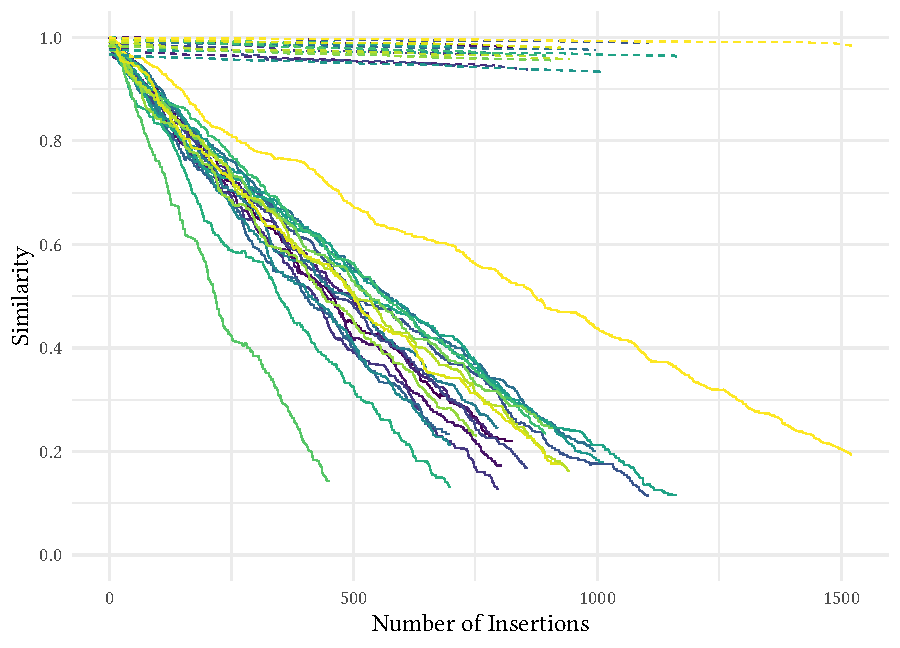
\includegraphics[width=1\linewidth]{figures/eval-tsn-steps.pdf}
    \caption[Impact of Token Sequence Normalization]{Similarities calculated by JPlag for obfuscated programs of a real-world introductory programming assignment dataset with an average of 1529 lines of code (LOC) per program via step-wise statement insertion as obfuscation attack. Each line represents a program, solid lines for JPlag as the baseline, and dashed lines are for JPlag with token sequence normalization.}
    \label{fig:tsn-impact}
\end{figure}

To assess the performance implications of our mechanism, we compared the runtime of JPlag with and without our approach.
We measured the runtime for two real-world datasets. We employed a consumer notebook, specifically a MacBook Pro equipped with an M1 Pro chip and 16GB of memory, for our performance measurements to provide a realistic environment.
As shown in \autoref{fig:tsn-runtime}, there is only an overhead of 0.89 seconds for one dataset and 6.45 seconds for the other. Note that this is the overhead for the complete datasets, not individual programs. State-of-the-art software plagiarism detectors like JPlag are highly optimized, and the performance impact of our mechanism is negligible. Thus, the total runtime of JPlag combined with our mechanism is mere seconds.

    \begin{table}
	\centering
	\begin{tabular}{llrrr}
		\toprule
		  Dataset Name & Metric     & JPlag     & JPlag with TSN & Difference\\
		\midrule
		\multirow{ 2}{*}{TicTacToe} & Runtime    & 6.97s     &    7.86s   & +0.89s\\
        %         &Relative Runtime   & 100.0\% &    112.7\% &\\ % with exact measurements it's . 7
	               &  $\sigma$ (SD)    & 0.10s     &    0.10s &+0.00s\\
        \hline 
        \multirow{ 2}{*}{BoardGame}   & Runtime          & 16.83s     &    23.28s   & +6.45s\\
		              & $\sigma$ (SD)    & 0.53s      &    0.44s    & -0.09s \\
		\bottomrule
    \end{tabular}
    \caption[Runtime Overhead of Token Sequence Normalization]{Runtime overhead of JPlag with token sequence normalization for two introductory programming assignment dataset TicTacToe (626 programs, 167.562 LOC total, \textasciitilde200.000 comparisons) and BoardGame (434 programs, 685.730 LOC total, \textasciitilde94.000 comparisons), avg. of 100 runs.}
	\label{fig:tsn-runtime}
    \end{table}
    

\subsection{Limitations}\label{sec:tsn-limits}

While token sequence normalization is a highly effective defense mechanism against insertion-based obfuscation attacks, it does have certain limitations. In the following, we discuss its dependence on the quality of the extracted semantic information and its applicability to other programming paradigms.

\subsubsection{Dependence on Semantic Information Extraction}
Token sequence normalization requires accurate extraction of semantic information during the tokenization step of the plagiarism detector. This semantic information, such as dependencies between tokens, is used to construct the token normalization graph. As previously discussed, this extraction process introduces a small degree of language dependence, as it must be tailored to capture critical relationships within the syntax and semantics of each programming language.
%
Although token sequence normalization overall is language-agnostic in its core design, its effectiveness depends on the quality and accuracy of this language-specific semantic information. We employ a conservative approach and thus only normalize the parts of the token sequence where tokens can be safely reordered or removed, making over-normalization not a problem as long as the extracted semantic information is correct.

However, if not enough semantic information is extracted, for example, only for some program elements, then the effectiveness of the defense mechanism decreases. This does not reduce the overall detection quality; it just reduces the resilience against insertion-based obfuscation attacks. As an example, consider the language C++. For this language, the standards include several cases of undefined behavior. Furthermore, various syntactical variations can express the same program behavior. Finally, its syntax is generally considered very complex.

These aspects make it hard to cover all edge cases when designing the extraction of semantic information for a new language such as C++. The overlooked edge cases could then be exploited to reduce the effectiveness of the defense mechanism, allowing, for example, the insertion of certain dead statements that are not recognized as such.
%
However, even if some edge cases are overlooked, token sequence normalization will still provide significant resilience, thus making effective obfuscation challenging.

\subsubsection{Applicability for Other Language Paradigms}
While the approach for token sequence normalization is language agnostic, applying it to vastly different paradigms, such as purely functional programming languages, presents unique challenges. For languages like Haskell, statement inter-dependencies and control flow differ significantly from languages like Java, C++, or Python.

In functional languages, especially in pure functional ones like Haskell, there are no traditional control flow statements (e.g., loops or conditionals in the imperative sense) that token sequence normalization typically handles through dependency graphs. Functional programs often rely on recursive function calls and higher-order functions, which make token-based sequence normalization less straightforward since there are no explicit control structures to anchor the ordering of the token normalization graph.
%
Moreover, functional languages emphasize immutability and avoid side effects, so they do not use variable assignments or mutable state as imperative languages do. The dependency relationships that token sequence normalization relies on, such as variable flow edges $E_{vf}$ or variable order edges $E_{vo}$, would have limited or no applicability. Haskell, for example, uses function compositions, pure functions, and monads to handle effects and dependencies.
%
Additionally, token sequence normalization is designed to work on a statement-by-statement basis, but functional languages often treat functions or expressions as atomic units. For instance, Haskell functions are typically small, pure, and composable, and their order can frequently be rearranged without affecting program semantics. Thus, a token-based normalization approach, like token sequence normalization, must define meaningful reordering boundaries.

However, this limitation is a broader problem, as plagiarism detection support for functional languages is generally limited~\cite{Hage2013}. However, token sequence normalization applies to the most frequently taught programming languages and thus covers typical use cases for source code plagiarism detection (see \autoref{sec:survey}).

% -------------------------------------------------------------------
\endinput % EVERYTHING BELOW IS EXCLUDED!!!

\begin{table}
    \centering
    \caption{Comparison of the original and obfuscated token sequences with the obfuscated one after the two steps dead node removal and topological sorting \autoref{tab:codesnippet}.}
    \label{tab:tokensfull}
    \scriptsize
    \begin{tabular}{ccccc}
        \hline
        \# & \textbf{Original} & \textbf{Obfuscated} & \textbf{DN Removed} & \textbf{Top. Sorted} \\
        \hline
        1  & \scriptsize\texttt{method start} & \scriptsize\texttt{method start} & \scriptsize\texttt{method start} & \scriptsize\texttt{method start} \\
        2  & \scriptsize\texttt{variable}     & \scriptsize\texttt{variable}     & \scriptsize\texttt{variable}     & \scriptsize\texttt{variable}     \\
        3  &                                  & \scriptsize\texttt{\textbf{variable}}     &                                  &                                   \\
        4  & \scriptsize\texttt{loop start}   & \scriptsize\texttt{loop start}   & \scriptsize\texttt{loop start}   & \scriptsize\texttt{loop start}   \\
        5  & \scriptsize\texttt{variable}     & \scriptsize\texttt{variable}     & \scriptsize\texttt{variable}     & \scriptsize\texttt{variable}     \\
        6  & \scriptsize\texttt{apply}        & \scriptsize\texttt{\textbf{assignment}}   & \scriptsize\texttt{\textbf{assignment}}   & \scriptsize\texttt{apply}   \\
        7  & \scriptsize\texttt{assignment}   & \scriptsize\texttt{\textbf{apply}}        & \scriptsize\texttt{\textbf{apply}}        & \scriptsize\texttt{assignment}        \\
        8  & \scriptsize\texttt{loop end}     & \scriptsize\texttt{loop end}     & \scriptsize\texttt{loop end}     & \scriptsize\texttt{loop end}     \\
        9  & \scriptsize\texttt{method end}   & \scriptsize\texttt{method end}   & \scriptsize\texttt{method end}   & \scriptsize\texttt{method end}   \\
        \hline
    \end{tabular}
\end{table}
\section{Subsequence Match Merging}\label{sec:smm}
In this section, we introduce our second defense mechanism (\contribution{3.2}) called \textit{subsequence match merging} (SMM)~\cite{Saglam2024d}.
While there is some research to counteract such automated obfuscation attacks, these approaches face two crucial challenges~\cite{Saglam2024b}.
First, \textit{language-dependence}: Defense mechanisms are often highly language-specific, hindering straightforward generalization or transferability across different programming languages.
Second, \textit{attack-type-dependence}: Defense mechanisms are usually only tailored to one specific attack vector, thus lacking broad resilience. While highly efficient against the intended attacks, they provide little resilience for other attack types.
Thus, they serve little protection against unknown attacks. Such emerging attacks, however, constitute the most challenging scenarios.
However, with the recent rise of large language models and their \textit{commoditization} via tools like ChatGPT~\cite{ChatGPT}, addressing emerging attacks is more crucial than ever~\cite{ChatGPTGuide}. 

Given these challenges, we introduce a novel approach called subsequence match merging to bolster the obfuscation resilience of today's state-of-the-art software plagiarism detectors.
%
All obfuscation attacks, whether known or unknown, have to disrupt the matching of code fragments to be effective~\cite{DevoreMcDonald2020}. Thus, they must affect the detectors' internal program representation~\cite{Saglam2024b}.
%
To this end, obfuscation attacks try to alter the structural properties of a plagiarized program.
%
Our approach iteratively merges neighboring fragment matches in pairs of linearized programs according to a well-designed heuristic until no more neighboring pairs remain. This process effectively reverses the effects of obfuscation, enhancing the detection of obfuscated plagiarism while minimizing false positives.
%
As our approach operates solely on the internal linearized representations of programs, it is entirely language-independent and not limited to a single obfuscation attack type.
Thus, subsequence is not limited in its effectiveness to semantic-preserving or semantic-agnostic obfuscation attacks.
It is also capable of defending against semantic-deviating obfuscation attacks.
We thus provide a robust and versatile approach for a broad spectrum of known and unknown obfuscation attacks.

\begin{factsheet}{Overview: Subsequence Match Merging} 
    \begin{description}[style=multiline,leftmargin=5.5cm]
        \item[Core Principle] Revert Match Splitting Heuristically
        \item[Targeted Obfuscation Attack] Unspecified, Broad Resilience
        \item[Language Family] Programming and Modelling Languages
        \item[Language Dependence] Language-Independent
        \item[Performance Impact] Moderate
        \item[Main Scalability Determinant] Number of Matches
        \item[Integration Complexity] Low
    \end{description}
\end{factsheet}

\subsection{Targeted Obfuscation Attacks}

Subsequence match merging is an algorithm that heuristically searches among all matched subsequence pairs between two linearized programs to find \textit{neighboring} matches that can be merged into a single one, subsuming the (unmatched) gap between them. This is done iteratively until no more neighboring pairs are found. This approach effectively reverts the effects of obfuscation attacks on the linearized program.
As discussed in \autoref{cha:threatmodel}, all obfuscation attacks must affect the token sequence, thus interrupting the matching, to be effective. 

Subsequence match merging relies solely on matching subsequences in the internal token-based representation, independent of the underlying programs. This makes it inherently language-independent. Furthermore, our approach relies only on the structural properties of all matched subsequences but does not consider the semantics of the corresponding tokens, thus making it attack-type-independent.
Therefore, our approach provides resilience against any potential obfuscation attack.
Consequentially, this subsequence match merging does not target a specific attack type. Instead, it aims to provide broad resilience that can be layer with other defense mechanisms.
In detail, it offers significant resilience against weaker obfuscation attacks and some resilience against stronger obfuscation attacks.

As discussed, all token-based plagiarism detectors employ a cut-off threshold, below which matched code fragments are ignored to avoid false positives. This threshold, often called minimum match length (MML)~\cite{Saglam2022}, defines the minimal number of tokens required for two matching subsequences to be counted toward the similarity score.
Thus, the minimum match length controls the sensitivity of the comparison algorithm: if set too low, it increases the similarity but also the likelihood of false positives and vice versa.
Obfuscation attacks affect the detection by splitting up matching subsequences of tokens until enough subsequences are small enough to fall below the minimum match length and are thus ignored.

Thus, our approach aims to reverse this by merging neighboring blocks of matches. The merging operates heuristically by assessing how close \textit{neighboring} matches are, regardless of whether the alterations initially involved insertion, deletion, or reordering. By carefully selecting the matches to merge, we ensure a negligible impact on the false positive rate.

\subsection{Neighboring Matches}
A key concept in our approach is \textit{neighborhood} of matches.
We define matches as neighbors if they directly follow each other in the same order in both token sequences of a program pair. \textit{Directly} refers to having no other matches in between on either side of the pair. This, however, does explicitly not include unmatched tokens.

\begin{theorem}[Neighboring Matches]\label{def:neighbors}
Let \( (t_i) \) and \( (t'_i) \) be the token sequences of two programs, and let \( (m_i) \) and \( (m'_i) \) be subsequences of matching tokens in \( (t_i) \) and \( (t'_i) \), respectively. Two matches \( (m_i) \) and \( (m'_i) \) are considered neighbors if:
\begin{align*}
(m_i) \sqsubseteq (t_i), \quad (m'_i) \sqsubseteq (t_i), \quad (m_i) \sqsubseteq (t'_i), \quad (m'_i) \sqsubseteq (t'_i),
\end{align*}
and
\begin{align*}
(m_i) \prec_{(t_i)} (m'_i), \quad (m_i) \prec_{(t'_i)} (m'_i),
\end{align*}
where \( \prec \) denotes the canonical order of subsequences in a token sequence. Specifically, it indicates the natural order based on the indices of the tokens within their respective sequences.
\end{theorem}

\begin{figure}[b]
    \centering
    
\includegraphics[width=\linewidth]{figures/algorithm/neighbors.pdf}
    \caption[Neighboring Subsequence Matches]{Two tokenized programs with four subsequence matches $(a_i)$--$(d_i)$, of which only the matches $(c_i)$ and $(d_i)$ are neighbors.}
    \label{fig:neighbors}
\end{figure}

To illustrate \autoref{def:neighbors}, \autoref{fig:neighbors} depicts four matches between the token sequences of two programs. The matched subsequences are in the order $((a_i), (b_i), (c_i), (d_i))$ in the original program and $((b_i), (a_i), (c_i), (d_i))$ in the variant. Therefore, matches $(a_i)$ and $(b_i)$ would not be considered neighbors, as their subsequence order is inconsistent across both programs. Matches $(a_i)$ and $(c_i)$ are not neighbors, as the corresponding subsequences in the original are interrupted by match $(b_i)$, which also is the case for $(b_i)$ and $(c_i)$ in the variant. In contrast, match $(c_i)$ and match $(d_i)$ are considered neighbors because they follow each other in the same order and are only separated by non-matching tokens.

Neighboring subsequence matches represent matching code fragments in the original programs. For instance, in \autoref{tab:running-example}, lines 1--3 and 6--8 match in the original program and in the variant. These lines appear in the same order and have no other matching segments in between, thus leading to a pair of neighboring matches in the token sequences. The non-identical statements that separate these neighboring matches are the inserted line 4 and the altered line 5.
%Neighboring token matches thus represent matching code fragments separated by non-identical statements.

\subsection{Algorithm}
\label{subsec:smm-algorithm}
Subsequence match merging operates as outlined in \autoref{alg:matchMerging}. The algorithm takes the token sequences of two programs and their matching subsequences as input. Note that this includes all matches, including those who fall below the minimal match length of the plagiarism detector. Initially, we compute which matching subsequences qualify as neighboring matches. If a pair of neighboring matches meets the merging criteria, we merge them and eliminate the gap in both token sequences.
This involves effectively ignoring the unmatched tokens between the neighboring matches. After each merge, we recompute the neighbors and repeat this process until no more neighboring matches that fulfill the merging criteria are found. This means that merged matches can be merged with others in the following iterations.
%
Our merging criteria are defined as follows:
\begin{description}[style=unboxed,leftmargin=0cm]
 \item[Minimal Neighbor Length:] Both neighboring matches must exceed a specific length in tokens (for example, matches with a length above two tokens).
 \item[Maximal Gap Size:] The mean gap of unmatched tokens between these neighboring matches must not exceed a specific size (for example, a gap below six tokens). 
\end{description}

More formally, we thus merge all neighboring merges where both thresholds mentioned above are fulfilled.
This is defined as follows.

\begin{theorem}[Neighbor Length Fulfillment]\label{def:neighbor-length}
Two neighboring matches \((a_i)_{i=1}^l\), \((b_j)_{j=1}^n\) according to \autoref{def:neighbors} and \autoref{def:matching-tokens} fulfill the minimal neighbor length threshold \(\ell_{\text{MNL}}\) iff
\[
    \ell_{\text{MNL}} \leq |a_i| = l \quad \land \quad \ell_{\text{MNL}} \leq |b_j| = n \,.
\]
\end{theorem}

\begin{theorem}[Gap Size Fulfillment]\label{def:gap-size}
Two neighboring matches \((a_i)_{i=1}^l\), \((b_j)_{j=1}^n\) according to \autoref{def:neighbors} and \autoref{def:matching-tokens}, which are separated in the token sequences of two programs by the subsequences \((c_k)_{k=1}^p\), \((d_m)_{m=1}^q\), fulfill the maximum gap size threshold \(\ell_{\text{MGS}}\) iff
\[
    \ell_{\text{MGS}} \geq \frac{|c_k| + |d_m|}{2} = \frac{p + q}{2} \,.
\]
\end{theorem}


\begin{algorithm}
\caption{Subsequence Match Merging}\label{alg:matchMerging}
\begin{algorithmic}[1]
  \Require{$tokenSequences, originalMatches$}
  \State $matches \gets originalMatches$
  \State $neighbors \gets \textproc{computeNeighbors}(matches)$
  \State $numberOfMerges \gets 0$
  \Repeat
    \For{each $neighborPair \in neighbors$}
      %\If{$\text{average size of } gapTokens \leq gapSizeThreshold$}
      \If{$\textproc{satisfiesMergingCriteria}(neighborPair)$}
        \State $mergedMatch \gets \textproc{mergeNeighbor}(neighborPair)$
        \State $matches \gets matches \cup \text{mergedMatch}$
        \State $matches \gets matches \setminus \text{neighborPair}$
        \State $numberOfMerges \gets numberOfMerges +1$
      \EndIf
    \EndFor
    \State $neighbors \gets \textproc{computeNeighbors}(matches)$
  \Until{no more valid merges}
  \If{$numberOfMerges \geq minimumMerges$}
    \State \Return $\textproc{pruneMatches}(matches)$
  \Else
    \State \Return $originalMatches$
  \EndIf
\end{algorithmic}
\end{algorithm}

Our algorithm merges pairs of neighboring matches when both have sufficient lengths and are separated by minimal tokens, indicating the pair represents a formerly single uninterrupted match. Our heuristic is based on thresholds for minimum neighbor length and maximum gap size, merging matches that meet these criteria.
Note that the neighbor length fulfills a purpose similar to the minimal match length. It controls the sensitivity of the approach.
%
After merging, we need to filter any remaining matches that fall below the minimum match length to ensure that the resulting matches do not violate the assumptions of the plagiarism detector. This means some merged matches must not be included, as they may fall below the minimum match length threshold (\textproc{pruneMatches} in \autoref{alg:matchMerging}).
By considering matches below the minimum match length threshold before the pruning step, our approach can merge matches that the plagiarism detector would not have considered. Essentially, this allows the fragmentation of matches to be reversed, thus reverting the effects of obfuscation attacks.
Finally, we check how many neighboring matches were merged. When this number is below a threshold called \textit{minimal merges} (MM), the merged matches are dropped, and the original ones are used. This threshold is a safeguard to reduce the impact on pairs or unrelated programs.

\autoref{fig:fullMatchMerging} illustrates the subsequence match merging algorithm as defined in \autoref{alg:matchMerging} for our running example in \autoref{tab:running-example}. It shows how the token sequences of two programs are aligned via subsequence match merging in two steps. 
\textit{Step 0} displays the token sequences of the original program and its obfuscated variant from \autoref{tab:re-tokens}, along with the matching subsequences between them. For illustrative purposes, let the minimum match length threshold be four tokens, resulting in a similarity score of 0\% because all three matches fall below this threshold.
Due to obfuscation, the matching subsequences are interrupted, and all matches fall below the minimum match length and are thus omitted.
In step 1, we merge the first two subsequence matches, which are only separated by a single token in the variant sequence. Both matches are at least two tokens long and only separated by \(\frac{0 + 1}{2} = 0.5\) tokens.
After merging, the match length increases to 5, thus raising the similarity score to 58.8\%.
In \textit{Step 2}, we assess the remaining pair of neighbors which also meet the threshold criteria.
We merge the remaining two subsequence matches, which are now separated by a single token in the original sequence. Again, both matches are long enough and are only separated by \(\frac{1 + 0}{2} = 0.5\) tokens. Since we cannot find any more matches to merge, we terminate. As we eliminate the separating tokens during the merging, the resulting match is above the minimal match length, and the token sequences of both programs are now considered identical.
Merging them raises the similarity score to 100\%, thus reverting the obfuscation demonstrated in the running example.

\begin{figure}
\centering
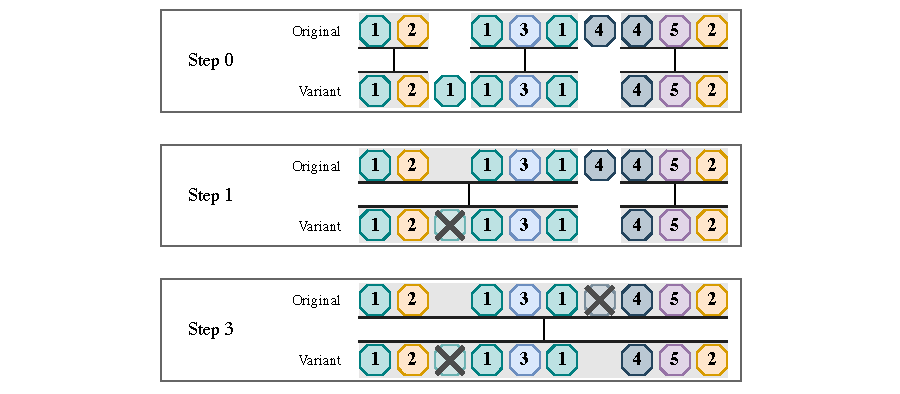
\includegraphics[width=\linewidth]{figures/algorithm/steps.pdf}
\caption[Subsequence Match Merging Example]{Steps of the subsequence match merging for the running example in \autoref{tab:re-tokens} (minimum match length = 4, minimum neighbor length =, 2 and maximum gap-size = 1).}
\label{fig:fullMatchMerging}
\end{figure}

\subsection{Complexity}
The runtime complexity of the \textit{Subsequence Match Merging} algorithm depends on the number of matches $m$ and the efficiency of merging operations.
The runtime complexity depends on the three main operations: Neighbor computation, merging, and pruning.
The neighbor computation scans all matches sequentially to identify adjacent pairs with a $O(m)$ complexity.
Merging a pair of neighbors is an $O(1)$ operation, while pruning matches after all iterations also requires $O(m)$ time.
We check each neighboring pair for the merging criteria and repeat this until no more merges occur.

In the worst case, each algorithm iteration performs an $O(m)$ neighbor computation and processes up to $O(m)$ merges, with a maximum of $m$ iterations if only one merge occurs per iteration. This results in a worst-case complexity of $O(m^2)$. Conversely, in the best case, where merges significantly reduce the number of matches (e.g., halving the matches in each iteration), the algorithm performs $O(\log m)$ iterations, with each iteration requiring $O(m)$ operations for neighbor computation and merging. Consequently, the best-case complexity is $O(m \log m)$.

The length of the token sequences limits the number of matches. For the sake of the complexity, $m$ can thus also be seen as the length of the longer sequence. As the worst-case runtime complexity for greedy string tiling per program pair is \( O(m^3) \) (see \autoref{sec:found-jplag}), subsequence match merging does not increase the runtime complexity of the plagiarism detection process.

\subsection{Hyperparameters}
To fine-tune the algorithm, we provide two primary hyperparameters: the minimum neighbor length and the maximum gap size (see \autoref{subsec:smm-algorithm}). These can be adjusted to, for example, fit the algorithm to a specific dataset.
Both thresholds are critical for tuning the heuristic's aggressiveness in deciding which neighboring matches to merge. Setting a low neighbor length and a high gap size threshold tends to merge unrelated matches, increasing false positives. Conversely, a high neighbor length and a low gap size limit the effectiveness of our approach by failing to detect most instances of plagiarism. 

We conducted a grid search for a suitable default parameterization to address the trade-off between precision and recall.
We explored neighbor length values from 1 to the minimum match length. The minimum match length was chosen as the upper threshold, as matches above this threshold have already been detected. Furthermore, we explore gap size values from 1 to 20. We chose 20 as the upper threshold, representing a significant code fragment. During our grid search, this was confirmed, as the best results occur far below the threshold of 20. After evaluating each combination across various real-world datasets consisting of different assignment types, sizes, and different programming languages, as well as with varying obfuscation attacks, we observed that a minimum neighbor length of 2 and a maximum gap size of 6 yields the strongest resilience against obfuscation attacks.
To recap, this means that neighboring matches are merged only if each match spans at least two tokens and six or fewer tokens separate them.
Thus, we propose these values as default parametrization. However, we also recommend adjusting these hyperparameters for the dataset at hand when using our approach.

Finally, for the number of minimal merges, we recommend a low value of between three and five. By choosing a conservatively low value here, we ensure that this safeguard does not affect the performance of the algorithm for obfuscated programs.

\subsection{Observed Impact}\label{sec:smm-impact}
This section presents initial observations on the effectiveness of subsequence match merging based on real-world data. It is important to note that this is not intended as a comprehensive evaluation but aims to provide an empirical perspective on how the defense mechanism performs in practical scenarios.

When applying subsequence match merging to an exemplary dataset from programming assignments and analyzing its impact, we observe a distinct difference between unrelated program pairs and those where one program was plagiarized and obfuscated to create the other. For instance, in cases of obfuscation through statement insertion using PlagGen~\cite{Broedel2023}, unrelated program pairs experience an average of 3.64 individual merges. In contrast, plagiarism pairs undergo an average of 73.90 merges. This indicates that the merging criteria of the algorithm rarely fulfilled for unrelated solutions but frequently fulfilled for plagiarism pairs, demonstrating the effectiveness of our heuristic. For this exact purpose, we designed the safeguard via a minimal number of merges. 

%\todo{Empiric results PP-19:}
%\todo{27 Plags: MaxGap{count=1552, sum=4945, min=1, average=3,186211, max=12}}
%\todo{351 Unrelated: MaxGap{count=1276, sum=3272, min=1, average=2,564263, max=12}}
%\todo{Means 73.90 individual merges per plag pair but only 3.64 for unrelated pair}

When varying the hyperparameters of the SMM algorithm for the aforementioned dataset, we can observe how the parameterization affects the effectiveness of the algorithm.
\autoref{fig:mm-nl} illustrates this for a varying minimal neighbor length. As previously discussed, this controls how long neighboring matches must be to qualify them for merging. The original and plagiarized programs achieve almost identical similarity values without match merging. The lower the minimal neighbor length, the clearer the separation becomes. We can see how this parameter controls the aggressiveness of the merging. Lower values lead to fewer individual merges and vice versa.

Next, \autoref{fig:mm-nl} illustrates the impact of the hyperparameters for a varying maximal gap size. The gap size controls how many tokens can separate two neighboring matches to still qualify them for merging. Again, without merging, the similarity values collapse. For the gap size, the effectiveness increases when increasing the parameter. However, the effects are less strongly pronounced compared to the neighbor length. Furthermore, the impact of an increasing gap size stagnates at a particular value. In the case of \autoref{fig:mm-nl}, this happens at a gap size of 5 tokens.

In Summary, we can observe that subsequence match merging increases the similarity of plagiarism pairs while maintaining a minor impact on the original and unrelated pairs. With this, subsequence match merging improves the resilience against obfuscation attacks.


\begin{figure}[p]
\centering
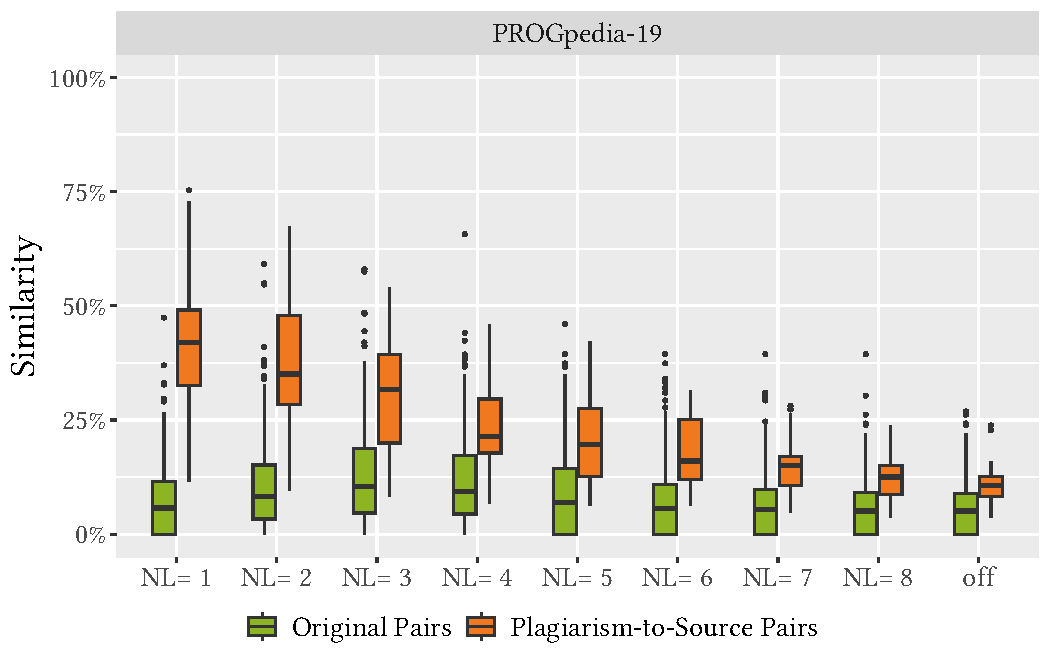
\includegraphics[width=0.95\linewidth]{figures/algorithm/eval-mm-NL_avg.similarity.pdf}
\caption[Impact of the Neighbor Length]{Impact of the hyperparameter neighbor length (NL) for a programming assignment dataset~\cite{paiva2023} and plagiarized programs via insertion-based obfuscation via PlagGen~\cite{Broedel2023}. Plagiarism pairs should be high, while original pairs should be low.}
\label{fig:mm-nl}
\end{figure}

\begin{figure}[p]
\centering
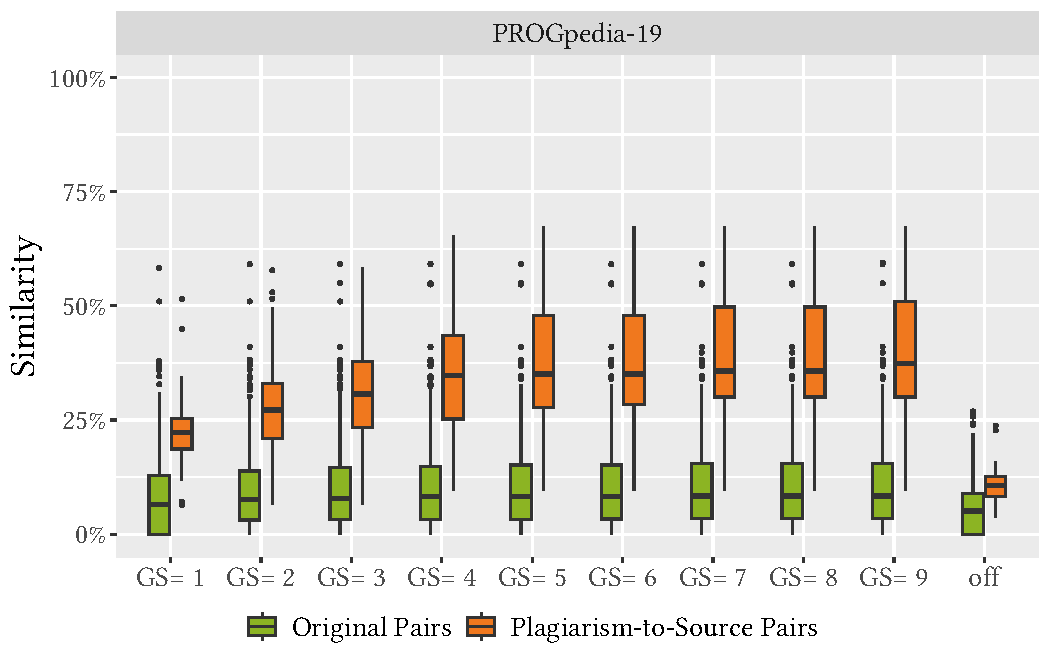
\includegraphics[width=0.95\linewidth]{figures/algorithm/eval-mm-GS_avg.similarity.pdf}
\caption[Impact of the Gap Size]{Impact of the hyperparameter gap size (GS) for a programming assignment dataset~\cite{paiva2023} and plagiarized programs via insertion-based obfuscation via PlagGen~\cite{Broedel2023}. Plagiarism pairs should be high, while original pairs should be low.}
\label{fig:mm-gs}
\end{figure}


\subsection{Limitations}\label{sec:smm-limits}

While subsequence match merging is an effective defense mechanism against various obfuscation attacks, there are some limitations to consider. In the following, we discuss the heuristic nature of the defense mechanism and the choice of suitable hyperparameter values.

    \subsubsection{Heuristic-based Defense}
    The strength of subsequence match merging is that it employs a heuristic to determine which matches to merge.
    Thus, it can provide broad obfuscation resilience, as it requires no knowledge of the specifics of obfuscation attacks.
    However, employing heuristics carries an inherent risk of increasing similarity for unrelated programs, as merging unrelated matches can inadvertently connect unrelated code fragments. This can be the case when a pair of unrelated programs has two sections that are coincidentally similar, and which are separated by a few lines of code in one or both of the programs that are not similar.
    To minimize the impact of match merging on pairs of unrelated programs, we use the original matches whenever too few merging operations are conducted. This significantly reduces the effect on unrelated programs, as for obfuscated programs, many merging operations occur (for example, three to four merges for unrelated programs versus 74 for obfuscated ones, as discussed in \autoref{sec:smm-impact}). 
    Although this mechanism minimizes false positives, subsequence match merging may still slightly increase the similarity of unrelated program pairs.

    \subsubsection{Choice of Hyperparameters}
    We intentionally avoided designing a defense mechanism that relies on too many hyperparameters, as it is always challenging for users to determine an optimal configuration in such cases~\cite{Schmid2022}.
    However, subsequence match merging relies on two hyperparameters (minimum neighbor length and maximum gap size) to determine which subsequences to merge. With a lower minimum neighbor length and a larger maximum gap size, the defense mechanism can revert the effects of stronger obfuscation attacks. However, it is also more prone to merging subsequences that do not belong together, meaning their corresponding code fragments are separated by correctly unmatched code (see \autoref{sec:smm-impact}).
    Incorrect parameter tuning could lead to missed plagiarism cases (under-merging) or excessive false positives (over-merging). To address this issue, we conducted a systematic hyperparameter search on different datasets. We observed that for our datasets, the effects of the hyperparameters are not strong enough to make under-merging or over-merging a probable issue. Specifically, we observed that the hyperparameters mainly affected how well the defense mechanism performed, but the overall detection quality did not fall below the base case, with subsequence match merging disabled.
    From this hyperparameter search, we derived recommended default values for the hyperparameters.
    While these values work well for various datasets, one limitation is that these values are not guaranteed to work for all datasets.
    However, as they are hyperparameters, they can be adapted to the specific dataset at hand.
    
\section{Model Subtree Reordering}\label{sec:msr}
In this section, we introduce our third defense mechanism (\contribution{3.3}) called \textit{model subtree reordering} (MSR)~\cite{Saglam2024a}. 
%
% MOTIVATON
Modeling assignments, such as \ac{UML} class, use case, sequence, and activity models, are common in computer science education~\cite{Ciccozzi2018, Saglam2023}. Modeling is integral to traditional software engineering courses due to the practical use of modeling languages like \ac{UML}. Furthermore, metamodeling assignments are becoming increasingly prevalent with the growing adoption of model-driven techniques~\cite{Brambilla2017, Hutchinson2011}. The complexity of modeling assignments and their demand for domain understanding and problem-solving skills make them susceptible to plagiarism~\cite{Martinez2020}. However, research on detecting plagiarism in modeling assignments is limited~\cite{Martinez2020, Saglam2022, Saglam2023}.

% REQUIREMENT: DEGREES OF FREEDOM
Effective plagiarism detection for modeling assignments necessitates mechanisms to handle degrees of freedom in models. Reordering attacks might exploit this flexible nature of models, which can lead to significant variations in the token sequence extracted from these models. While token-based detection approaches can detect large-scale reordering, for example, reordering methods in a class or classes in a \ac{UML} diagram, they are vulnerable to fine-grained reordering attacks~\cite{Saglam2022}. For program code, statements have a strong interdependence, thus limiting the effectiveness of reordering attacks (realistically, such an obfuscation attack will only reduce the similarity by about five percentage points~\cite{Saglam2024b}). For modeling artifacts, however, these fine-grained reordering attacks can effectively obfuscate plagiarism.
%
% EXAMPLE OF THIS
For example, the order of elements within multi-valued containment references can vary significantly in \ac{EMF} metamodels.
Likewise, in \ac{UML} class models, the order of attributes and methods within a class is often flexible and does not affect the model's semantics. Similarly, the sequence of states and transitions is not semantically significant in state charts. Instead, the critical aspect is the specific state from which a transition originates and the state to which it leads.
%
In the following, we discuss the targeted obfuscation attacks, the fundamental concept of model subtree reordering, the detailed algorithm, its complexity, and the limitations of the defense mechanism.

\begin{factsheet}{Overview: Model Subtree Reordering} 
    \begin{description}[style=multiline,leftmargin=5.5cm]
        \item[Core Principle] Normalize the Order of Elements in the Model
        \item[Targeted Obfuscation Attack] Model Element Reordering
        \item[Language Family] Modelling Languages
        \item[Language Dependence] Language-Agnostic
        \item[Performance Impact] Very Low
        \item[Main Scalability Determinant] Size of Input Models
        \item[Integration Complexity] Moderate
    \end{description}
\end{factsheet}

\subsection{Targeted Obfuscation Attacks}
When using token-based approaches for modeling plagiarism detection, obfuscation attacks based on moving and swapping elements on a fine-grained level pose a viable threat~\cite{Saglam2022} because of the degrees of freedom discussed above.
Consider the view on the \texttt{Store} package in \autoref{fig:example-view}. It depicts two classes with their corresponding attributes, references, and containment references.
For this model view, \autoref{tab:example-view} presents three corresponding token sequences. All three sequences correctly represent the same model elements depicted in \autoref{fig:example-view}. However, the order of tokens varies between the sequences.
The original sequence represents the element order as shown in the graphical view. The first variant is created by swapping the tokens corresponding to each class, slightly altering the token sequence. The second variant is created from the first by reordering the tokens of the features, again modifying the token sequence order completely.
%
These variations in token sequences are a form of obfuscation where the token sequence remains semantically equivalent, but its representation is altered. This is possible for \ac{EMF} or \ac{UML} models, as the order of classes in a package and the order of features in a class have no semantic relevance. This also applies to many other modeling languages. Reordering is also common in source code plagiarism, but there, it provides limited effectiveness~\cite{Saglam2024b}.

Model subtree reordering targets the unique challenges posed by ordering-based obfuscation attacks on modeling artifacts.
To reduce the impact of the degrees of freedom common in modeling artifacts, we normalize the order of tokens corresponding to the elements in the model, ensuring a consistent representation of modeling artifacts and thereby countering obfuscation efforts that rely on the fine-grained reordering elements.
However, normalization in this context is far from trivial.
The properties used for normalization must be selected carefully to avoid introducing new attack vectors, and the process must minimize changes to the token sequence to prevent false positives.
Only \textit{robust} criteria can provide stability and invariance to obfuscation attacks.

\begin{samepage}
\begin{figure}[b]
    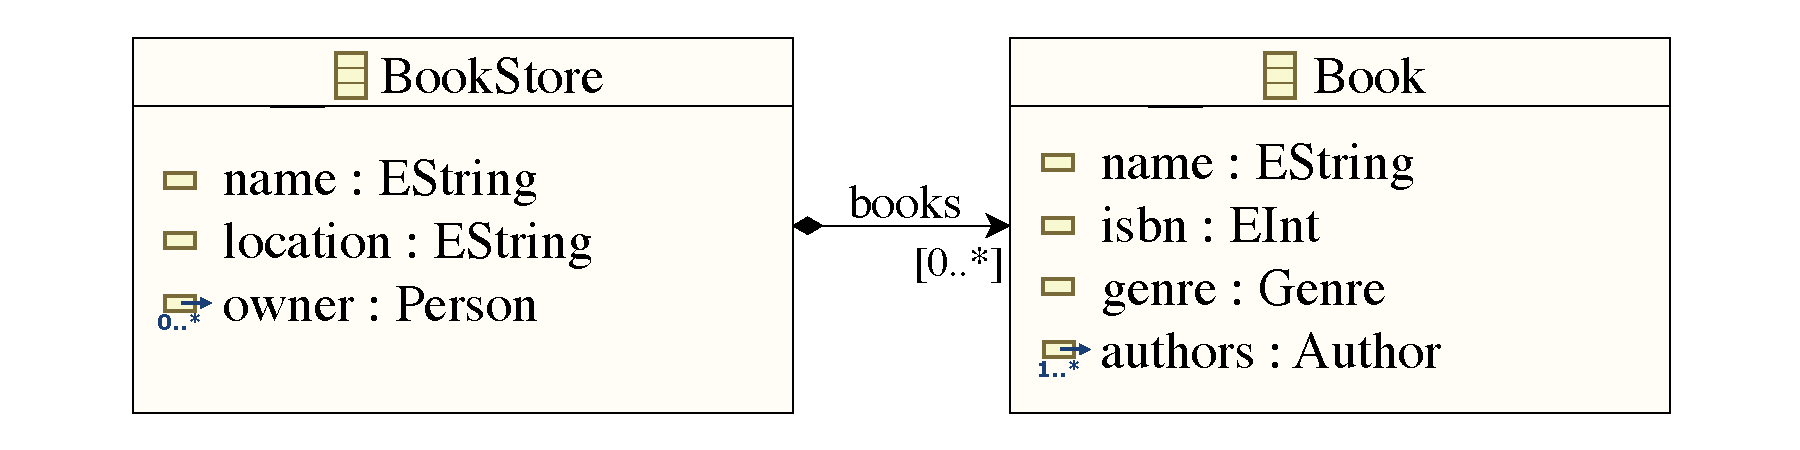
\includegraphics[width=\textwidth]{figures/mde/bookstore-view.pdf}
    \caption[Bookstore Model View]{View on the package \texttt{Store} of the second bookstore management system model as shown in \autoref{fig:running-example}, depicting two classes with their attributes and references.}
    \label{fig:example-view}
%\end{figure*}
\end{figure}

\begin{table}[b]
    \centering
    %\small
    \begin{tabular}{clll}
		\toprule
		\# & \textbf{Original}     & \textbf{Variant 1}    & \textbf{Variant 2}    \\
		\midrule
		1  & \texttt{Class}        & \texttt{Class}        & \texttt{Class}        \\
		2  & \texttt{ Containment} & \texttt{ Attribute}   & \texttt{ Attribute}   \\
		3  & \texttt{ Attribute}   & \texttt{ Attribute}   & \texttt{ Reference}   \\
		4  & \texttt{ Attribute}   & \texttt{ Attribute}   & \texttt{ Attribute}   \\
		5  & \texttt{ Reference}   & \texttt{ Reference}   & \texttt{ Attribute}   \\
		6  & \texttt{Class End}    & \texttt{Class End}    & \texttt{Class End}   \\
		7  & \texttt{Class}        & \texttt{Class}        & \texttt{Class}    \\
		8  & \texttt{ Attribute}   & \texttt{ Containment} & \texttt{ Attribute}   \\
		9  & \texttt{ Attribute}   & \texttt{ Attribute}   & \texttt{ Reference} \\
		10 & \texttt{ Attribute}   & \texttt{ Attribute}   & \texttt{ Containment}   \\
		11 & \texttt{ Reference}   & \texttt{ Reference}   & \texttt{ Attribute}   \\
		12 & \texttt{Class End}    & \texttt{Class End}    & \texttt{Class End}    \\
		\bottomrule
    \end{tabular}
    \caption[Example Obfuscation: Reordering]{Three token sequences, all representing the model view depicted in \autoref{fig:example-view}. The original reflects the element order of the view, while the first variant is created by swapping the tokens of each class, and the second variant is created from the first by reordering the tokens of the features. Note that all references are multi-valued, which is omitted for readability.}
    \label{tab:example-view}
\end{table}
\end{samepage}

Simple approaches like sorting by type or lexical order are insufficient, as they can be easily manipulated by specific obfuscation attacks (e.g., element insertion or property changes). The normalization is either ineffective or can be affected via specific obfuscation attacks.
For example, consider a hypothetical normalization based on element names: Whenever named model elements can be in an arbitrary order, they are sorted lexically via their names. While this provides resilience against reordering, it also includes vulnerability against renaming, as minor name changes now affect the element order. Besides names, other vulnerable properties include identifiers, data types, values, and other literals.
Normalization properties must be stable, invariant, and meaningful to detect plagiarism accurately and effectively.
Thus, robust properties are only based on the information already used by the plagiarism detectors and are limited to the extracted tokens corresponding to the patterns and structural patterns in these tokens.


\subsection{Concept}
As discussed in \autoref{sec:mde-approach}, tokenization references refer to the meaningful connections between elements in a model that capture the underlying semantics of the modeled system. Unlike syntactic references, which focus on the structural aspects of the model, tokenization references emphasize the relationships and dependencies that convey the intended behavior and functionality. 
Again, consider a state chart model. While structurally, all states might be contained under a common root element, these containment references are syntactic references. The underlying semantics are modeled by transition references between states, which are thus considered tokenization references.
These references are crucial for accurately detecting plagiarism in modeling assignments, as they ensure that the detection mechanisms account for the intent and semantics behind the models rather than just superficial similarities. By leveraging tokenization references, we can improve the robustness of modeling plagiarism detection. However, this also means these tokenization references must be identified for each modeling domain, as this distinction is purely conceptual and not reflected in the actual modeling artifacts.

Model subtree reordering is designed against reordering attacks by specifically leveraging these tokenization references to normalize the order of the token sequence. 
The approach applies to any modeling artifact with a tree-like structure where tokenization references can be identified. However, the effectiveness of this method depends on the extent of variability allowed within these types of artifacts.
%
To ensure a deterministic order in the token sequences representing modeling artifacts, we sort the elements in each multi-valued tokenization reference first based on their token type and then based on the distribution of the tokens in their subtree of direct and indirect children.
While the former is a coarse-grained ordering criterion to group model elements that map to the same token type, the latter is a more fine-grained one to capture and preserve the structural nuances within subtrees of the referenced elements.

At a high level, our approach leverages the concept of token type vectors to represent the structure of the model subtree. These vectors capture the frequency of various token types within the subtree, allowing us to compare and sort elements based on their structural characteristics. Thus, such a vector represents the distribution of different kinds of model elements in a specific part of the model. For example, we can consider the three subtrees illustrated in \autoref{fig:tree-examples}. Note that these are token trees, meaning the structure defined by the tokenization references of a model where each model element is replaced by its corresponding token. While all three trees are similar, subtree A has a different distribution of tokens than subtrees B and C, as each type (represented by color) occurs only once. While the subtrees B and C are structurally different, they share the same distribution of tokens. Note that the tree B can be transformed into the tree B with a single reordering operation.

If we now interpret these vectors as points in a multi-dimensional space, we can use the distance of these points to estimate how structurally similar two parts of a model are. By finding a path (meaning a sequence that includes all points) in this space that minimizes the distance between points, we can derive an order that is both deterministic and not easy to affect intentionally. This approach ensures that structurally similar elements are consistently ordered, thereby mitigating the effects of obfuscation through reordering while maintaining the stability of the normalization process.


\begin{figure}
    \centering
    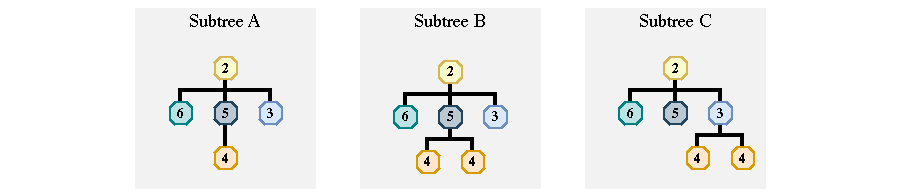
\includegraphics[width=\linewidth]{figures/mde/subtree-examples.pdf}
    \caption[Model Subtree Examples]{Three exemplary model subtrees based on tokenization references in token representation, where subtree A contains a slightly different token distribution than subtrees B and C, which share the same distribution.}
    \label{fig:tree-examples}
\end{figure}


\subsection{Algorithm}
Our normalization algorithm consists of several steps. The entire algorithm is listed in \autoref{alg:NormalizationAlgorithm}.
We begin by generating tokens for each element's subtree and then create a token type vector that indicates how often each type of token occurs within that subtree. For instance, in the case of the class \texttt{Book} depicted in \autoref{fig:tokenization}, this vector is represented as $[2, 1, 1, 0, \dots, 0]$, where the vector components correspond to two attributes, one identifier attribute, and one reference.
To enable meaningful comparisons between these vectors, we first normalize them. The normalization is done by computing the Euclidean norm of each vector:
\begin{align*}
    \|\mathbf{v}\|_2 = \sqrt{\sum_{i=1}^{n}v_i^2}
\end{align*}
This normalization process scales the vectors to have a length of 1, ensuring that the comparison between them is not influenced by the absolute magnitude of the original vectors but by the distribution of token types within each subtree.
Once normalized, these vectors can be interpreted as points in a multi-dimensional coordinate space, where each dimension corresponds to a specific token type. The position of each point in this space is determined by the distribution of token types in the corresponding element's subtree. For example, a vector with more attributes will be closer to the axis representing attributes.

To compare these points (representing different elements), we calculate the Euclidean distance between any two points $\mathbf{p}$ and $\mathbf{q}$ using the following metric:
\begin{align*}
    d_{\mathrm{E}}(\mathbf{p}, \mathbf{q}) = \sqrt{\sum_{i=1}^n (q_i-p_i)^2}.
\end{align*}
Using these distances, we construct a nearest neighbor path that sequentially connects each point to its closest neighbor, starting from the point associated with the element with the most tokens in its subtree. This ordering method prioritizes elements with greater structural complexity, which helps preserve the overall structure during the normalization process.
%
In cases where two or more points are equidistant from the last point in the path, we resolve the tie by referring to the original order of the elements. This ensures that the normalization process is stable, meaning that the same input will always produce the same normalized output, avoiding the introduction of inconsistencies due to random ordering.
%
%
Finally, to normalize the order of elements within a tokenization reference, we apply a two-step sorting process:
    \begin{enumerate}
        \item Primary Sorting by Token Type: We first sort the elements based on their token type vectors, providing a coarse-grained ordering that groups similar elements.
        \item Secondary Sorting by Nearest Neighbor Path: If two elements have identical token type vectors, we further sort them according to their position in the calculated nearest neighbor path. This fine-grained sorting helps maintain the relative order of structurally similar elements.
    \end{enumerate}
This approach ensures that the elements within a model are consistently ordered, thereby countering potential obfuscation strategies that rely on reordering elements.


\autoref{fig:tokentreenorm} illustrates the process of reordering tokens for three elements within the same (multi-valued) tokenization reference. The normed subtree vectors are used to calculate the elements' distances, sorting the elements according to the computed nearest neighbor path.
\begin{enumerate}
    \item {Token Tree}: We start with the token trees for three classes, each containing various tokens that represent different model elements such as identifiers, attributes, and references.
    \item {Subtree Vectors}: As a first step, the algorithm generates subtree vectors for each class, denoted as \( \mathbf{v}_a \), \( \mathbf{v}_b \), and \( \mathbf{v}_c \). These vectors count the occurrences of each token type within the subtrees. For example, the subtree vector for \texttt{Class} $a$ is \( \mathbf{v}_a = [1, 1, 0, \dots, 0] \), indicating one identifier and one attribute.

    \item {Normalized Vector}: Next, each subtree vector is normalized by its Euclidean norm \( \|\mathbf{v}\|_2 \). The normalized vectors represent the scaled distribution of tokens, ensuring comparability regardless of their original magnitude.

    \item {Euclidean Distance}: The normalized vectors are then used to calculate the Euclidean distance between each pair of elements. The distance matrix \( D \) encapsulates these distances, with each entry \( d_{ij} \) representing the distance between the vectors of \texttt{Class} $i$ and \texttt{Class} $j$. For example, the distance between \( \mathbf{v}_a \) and \( \mathbf{v}_b \) is \( d_{ab} = 0.765 \).

    \item {Nearest Neighbor Path}: Using the distance matrix \( D \), the algorithm determines the nearest neighbor path. The path starts from the element with the largest subtree (in this case, \texttt{Class} $b$) and proceeds by selecting the nearest neighbor at each step.

    \item {Normalized Token Sequence}: Finally, the model elements are reordered according to the nearest neighbor path, resulting in a normalized token sequence.
\end{enumerate}


\begin{figure}
    \centering
    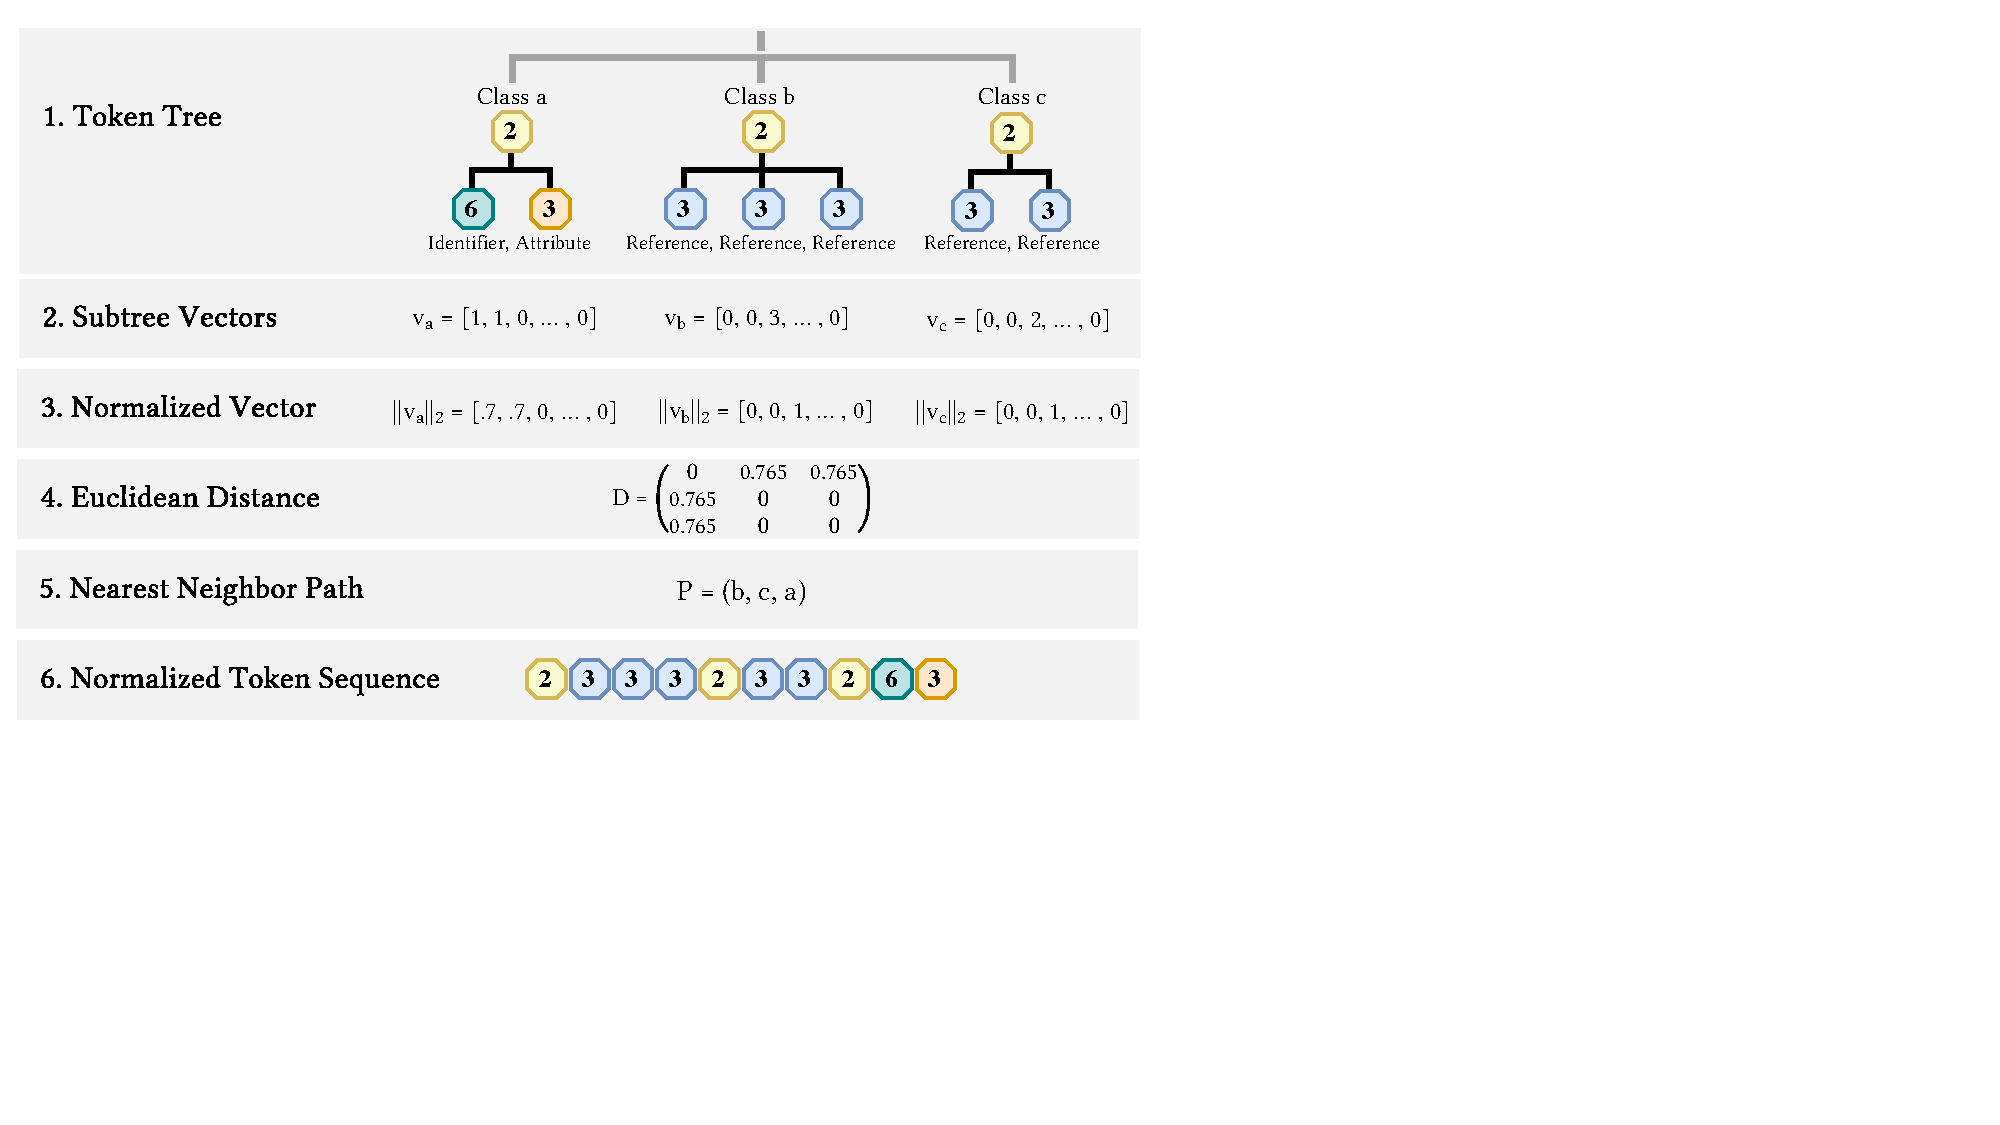
\includegraphics[width=0.9\linewidth]{figures/mde/normalization-new.pdf}
    \caption[Model Subtree Reordering Example]{Example illustrating how model subtree reordering normalizes the token sequence via element reordering for a multi-valued reference containing three classes.}
    \label{fig:tokentreenorm}
\end{figure}

\begin{algorithm}
    %\captionsetup{belowskip=-\baselineskip}
	\caption{Model Subtree Reordering}
	\label{alg:NormalizationAlgorithm}
	\begin{algorithmic}
		\Require{List of model elements $E$ with length $n$}
		\Function{Normalize Token Sequence}{$E$}
		\State{$V \gets$ empty list of vectors}
        \For{$e_i \in E$}
		      \State{$v_i \gets$ calculate token type vectors for subtree of $e_i$}
            \State{$v_i \gets$ euclidean norm $\|\mathbf{v_i}\|_2 $}
		\EndFor
  
        \State{$D \gets$ empty distance matrix with size $n \times n$ }
		\For{$v_i, v_j \in V$}
		      \State{$d_{i,j} \gets$ euclidean distance $d_{\mathrm{E}}({v_i}, {v_j})$}
		\EndFor
  
		\State{$v_{max} \gets$ vector in $V$ of element with largest subtree}
            \State{$P \gets$ nearest neighbor path for $D$ starting from $v_{max}$}
            \State{$S \gets$ sort $E$ by token type, if equal by position in $P$}
            \State{\Return{$S$}}
		\EndFunction
	\end{algorithmic}
\end{algorithm}

% OLD VERSIONS
%\input{tables/normalization}

\noindent

In our approach, we opted to use the nearest neighbor path rather than the shortest path, as the nearest neighbor path is more robust against modifications in the subtrees. The shortest path, which typically minimizes the total distance between points in a coordinate space, can be sensitive to even minor changes in the structure of the elements, potentially leading to significant shifts in the ordering. Such sensitivity would make the normalization less robust.

On the other hand, the nearest neighbor path focuses on maintaining local consistency by linking each point to its closest neighbor, regardless of the overall path length. This method ensures that small changes in the subtree structure do not disproportionately affect the overall sequence, making the path, and hence the normalization, more resilient to obfuscation techniques that involve subtree modifications.

We further enhance the robustness of the normalization by carefully choosing the starting point for constructing the nearest neighbor path. Specifically, we start from the element with the most tokens in its subtree. This choice is based on findings from our pre-study, which indicated that beginning with the most complex (or structurally significant) element leads to a normalization more resistant to reordering attacks. The rationale is that the element with the most tokens likely has a more pronounced impact on the overall model structure, making it a stable anchor for the normalization process.

Using the nearest neighbor path and selecting a strategic starting point, our approach effectively addresses the normalization challenge in modeling plagiarism detection. It ensures that similar structures are consistently ordered in a way that is less susceptible to manipulation. This combination of strategies—prioritizing local consistency and starting with the most significant element—provides a more stable and reliable method for detecting plagiarism in models.


\subsection{Complexity}
The runtime complexity of the model subtree reordering algorithm in \autoref{alg:NormalizationAlgorithm} depends on the tree defined by the tokenization references and is thus influenced by the size of the subtrees and the number of model elements. Note that a tree with $m$ nodes can have a maximum of $m$ subtrees when every node except the root is a leaf. Furthermore, the maximum number of tokens in a subtree is limited by $m$.

The runtime complexity of model subtree reordering depends on the three main operations: Calculating the token type vectors, computing the distance matrices, constructing the distance matrices, and sorting the subtrees via a nearest neighbor search.
%
For an entire model of $m$ elements, the token type vectors for each subtree can be calculated via a single depth-first search with the runtime complexity of $O(m)$.
Constructing the distance matrix involves computing pairwise distances for up to $m-1$ elements (when all model elements are leaves of a single root), which contributes $O(m^2)$ complexity.
Sorting of all elements according to their distances via a nearest neighbor search has a complexity of $O(m \log m)$.

The overall runtime complexity is thus $O(m^2)$.
As the worst-case runtime complexity for greedy string tiling per program pair is \( O(m^3) \) (see \autoref{sec:found-jplag}), model subtree reordering does not increase the runtime complexity of the plagiarism detection process.

\subsection{Limitations}\label{sec:msr-limits}
While model subtree reordering is a robust defense mechanism against reordering-based obfuscation attacks for modeling artifacts, it does have certain limitations. In the following, we discuss its dependence on tokenization references, the focus of the defense mechanism, and the effect on unrelated models.

%\begin{enumerate}
    \subsubsection{Dependence on Identifying Tokenization References} As our general approach to modeling plagiarism detection, model subtree reordering 
    depends on the modeling domain and language (see \autoref{sec:mde-limit-domain}). Model subtree reordering operates on stable tokenization references to establish a normalized order. For tree-based models like \ac{EMF} models or \ac{UML} class models, these tokenization references are the containment relations. However, identifying these references is not trivial for some modeling languages and may require domain-specific adjustments for different modeling languages (see \autoref{subsec:tokenization}). This dependency on domain knowledge limits the mechanism as it increases the complexity of applying it to new modeling languages. Nevertheless, this domain-specific adjustment is required to apply our detection approach in the first place and is, thus, no additional effort for model subtree reordering.
    
    \subsubsection{Focused Resilience} model subtree reordering is designed to mitigate reordering attacks by normalizing the token sequence based on model element distributions in subtrees. However, it does not provide resilience against other forms of obfuscation, such as inserting irrelevant model elements. %Such attacks can introduce variability that model subtree
    Although model subtree reordering leverages token subtree distributions, which are much more robust than simpler, vulnerable criteria (e.g., names), substantial modifications to specific parts of a model can still impact the normalization. Such modifications would require significant changes, such as inserting entirely new subtrees, rather than minor adjustments, like adding individual elements. The reason for this is the sorting via nearest neighbor paths, which is not affected by minor changes to the token vectors.
    Even with these large-scale modifications, the effect on obfuscation may remain limited, as inserting new subtrees only partially disrupts the ordering.
    To address cases where the normalization provided by model subtree reordering is affected, model subtree reordering can be combined with subsequence match merging, which combines focused and broad resilience.

    \subsubsection{Effect on Unrelated Models}
    Another limitation of model similarity reordering is that any normalization process can inadvertently increase the similarity of unrelated models. As a normalization technique seeks to resolve ambiguities and standardize representations, it may lead to a situation where models that initially exhibit different structures appear more similar due to the reordering.
    As for all normalization techniques, the question with model subtree reordering is how pronounced this effect is.
    As token subtree reordering is a very abstract technique that only considers the tokens themselves to limit itself to a robust normalization criterion, its normalization of the token order is very broad. In contrast, token sequence normalization only reorders tokens of statements that are not interdependent. Model subtree reordering generally reorders all model elements for each tokenization reference. Thus, it may also affect unrelated models.
    This issue may be less significant for larger models, as they generally produce larger token subtrees with a more complex token distribution. This complexity results in more unique vectors for reordering based on the nearest neighbor paths. In contrast, smaller models do not benefit from this complexity, making the effects of normalization on unrelated models potentially more pronounced.
  
\section{Exploring Additional Defense Mechanisms}\label{sec:other-defense}
This section briefly mentions additional defense mechanisms we explored alongside those mentioned in the previous sections. However, the now-mentioned defense mechanisms have limited language independence or do not fulfill the essential requirements defined in \autoref{sec:tsn-requirements}.
Despite these approaches not being the core contributions of this dissertation, we still want to provide an overview of them. %Furthermore, we compare them to our primary defense mechanisms.

\textbf{Structural Normalization via Code Property Graphs}~\cite{Maisch2024}: We explored an approach to extracting the token sequence of programs from code property graphs instead of parse trees. Before tokenization, we normalize the code property graphs via graph transformations to counter semantic-preserving refactoring-based obfuscation attacks.
This includes refactoring operations like extracting expressions as variables or constants, introducing constant container classes, swapping if-else statements and inverting the corresponding conditions, inserting methods and constructors, and introducing access methods for existing fields.
Similarly to tokens, the sequence normalization approach can also be used to normalize the order of statements and to remove dead code. This approach can be seen as an extension of token sequence normalization. However, it is entirely language-dependent, as tokenization is based on code property graphs, and the corresponding transformations have to be defined for each programming language.

\textbf{Normalization via LLVM IR}~\cite{Heneka2023}: LLVM uses an intermediate representation language resembling assembly code. LLVM supports transforming code in multiple languages into LLVM IR code. During this transformation, code can be heavily optimized. This includes, for example, dead code removal. We investigated plagiarism detection via this intermediate representation. While it does provide resilience for specific obfuscation attacks, it has some drawbacks. First, the LLVM IR code is platform-dependent; thus, the results vary depending on the system architecture. Second, only some languages are supported by LLVM. Finally, the visualization limits the approach, as it shows matches on the IR code. This approach resembles the approach proposed by \citet{DevoreMcDonald2020} of using assembly code for plagiarism detection.

\textbf{Compiler-based Preprocessing}~\cite{krieg2022}: Some compilers provide aggressive preprocessing techniques to optimize program code. This often includes dead code removal and could be used to reduce the impact of some obfuscation attacks. However, this is a pure pre-preprocessing technique (thus falling short for nearly all requirements defined in \autoref{sec:tsn-requirements}) that is strongly language-dependent and provides only limited resilience.

These defense mechanisms provide obfuscation resilience but have disadvantages regarding language dependence or the abovementioned requirements. In the following, we also mention two approaches that are not sufficiently effective in providing obfuscation resilience.

\textbf{Pre-matching Token Filtering}~\cite{krieg2022}: We explored an approach based on sliding windows that filter the token sequences before the actual subsequence matching to reverse the splitting of matches. This heuristic approach was computationally expensive and only somewhat effective when combined with other defense mechanisms. However, this approach inspired our approach of merging subsequence matches. Both approaches share that they are language-independent and attack-independent.
    
\textbf{Token Transformation Patterns}~\cite{krieg2022}: Here, we explored defining a set of token patterns based on the different token types that, if detected in a token subsequence, would lead to the removal of tokens. An example would be the removal of all tokens between a return statement and the end of a block or method. However, these patterns are strongly token-dependent and only provide resilience for specific obfuscation attacks. This only provides limited resilience even among a single attack type, such as insertion-based obfuscation.

\endinput



\begin{table}[b]
	\centering
	\footnotesize
	\begin{tabular}{p{4cm}ccccc}
		\hline
		Defense Mechanisms & Target & Lang.-Ind. & Eff. & Scope & Obfucations \\
		\hline
	    SMM & Both & ++ & ++ & Wide & Any \\ 
		TSN & Code & + & +++ & Narrow & Insertion, Reordering \\
		MSR & Models & + & ++ & Narrow & Reordering \\ 
		Intermediate Representation & Code & o & + & Wide-ish & Many \\ 
         \hline
		Code Property Graphs & Code & o & ++ & Narrow & Refactoring \\ 
		Compiler-based Pre-Processing & Code & $--$ & o & Narrow & Insertion \& Others \\ 
		Token Transformation Patterns & Code & $--$ & - & Narrow & Insertion \& Others \\
		Token Sequence Filtering & Both & ++ & o & Wide & Any \\
		\hline
	\end{tabular}
	\caption[Overview on All Defense Mechanisms]{TODO}
    \todo{TODO}
\end{table}
